\documentclass[aps,prb,superscriptaddress]{revtex4-2}
\usepackage{xcolor}
\usepackage{CJKutf8}
\usepackage{graphicx}
\usepackage{amsmath}
\usepackage{color}
\usepackage{braket}
\usepackage{caption}
\usepackage{bm}
\usepackage[colorlinks=true, letterpaper=true, pdfstartview=FitV, linkcolor=blue, citecolor=blue, urlcolor=blue]{hyperref}
% \usepackage{geometry}
% \geometry{a4paper,scale=0.8}

\captionsetup{font={scriptsize}}

% \begin{CJK}{UTF8}{gbsn}
\begin{document}

\title{Notes on quantum transport in mesoscopic systems}
\author{Li Gaoyang}
\date{2020/12/1}
% \date{\today}
\maketitle
\tableofcontents
% \newpage

\section{Basics}
\subsection{Magnon}
A magnon is a quasiparticle, a collective excitation of the electrons' spin structure in a crystal lattice. In the equivalent wave picture of quantum mechanics, a magnon can be viewed as a quantized spin wave. Magnons carry a fixed amount of energy and lattice momentum, and are spin-1, indicating they obey boson behavior.
\subsection{Hall effect}
\subsubsection{Conventional Hall effect}
\subsubsection{Quantum Hall effect}
\subsubsection{Spin Hall effect}
Occurs in paramagnetic systems as a result of spin-orbit interaction, refers to generation of pure spin current transverse to an applied electric field, even in the absence of magnetic field.

Similar to charge accumulation at sample edges in conventional Hall effect, spin accumulation is expected in spin Hall effect.
\begin{itemize}
\item extrinsic spin Hall effect: originates from asymmetric scattering for spin-up and spin-down.
\item intrinsic spin Hall effect: originates from band structures without scattering.\cite{ref1}
\end{itemize}
\subsubsection{Fractional Hall effect}
\subsubsection{Anomalous Hall effect}

\section{Spin current in NM/NM/FI system}
\subsection{Model Hamiltonion}
For system consists of non-magnetic metal (NM) region sandwiched by a left NM lead and a right ferromagnetic insulating lead (FI), the Hamiltonian is
\begin{align}
H&=H_{\rm L}+H_{\rm C}+H_{\rm R}+H_{\rm T}+H_{\rm sd}.\\
H_{\rm{L}} &= \sum_{k\sigma} (\varepsilon_{k\sigma}-\mu_{\sigma}) c_{k \sigma}^{\dagger} c_{k \sigma},\\
H_{\rm{C}} &= \sum_{n\sigma}\varepsilon_{\sigma} d_{n\sigma}^{\dagger} d_{n\sigma},\\
H_{\rm{R}} &\approx \sum_{q} \hbar w_{q} a_{q}^{\dagger} a_{q},
\end{align}
are Hamiltonians of left lead, central region and right lead respectively. $H_{\rm T}$ is the hopping between the left lead and the central region, while $H_{\rm sd}$ is the exchange coupling between right lead and central region,
\begin{align}
H_{\rm{T}} =& \sum_{nk\sigma}( t_{nk\sigma} c_{k \sigma}^{\dagger} d_{n\sigma} + t_{nk\sigma}^{*} d_{n\sigma}^{\dagger} c_{k\sigma}),\\
H_{\rm{sd}}=& -\sum_{q n n^{\prime}} J_{q n n^{\prime}} a_q^{\dagger} d_{n \uparrow}^{\dag} d_{n^{\prime} \downarrow} +\text { h.c. }
\end{align}
Here $S_{q}^{-} \approx \sqrt{2 S_{0}} a_{q}^{\dagger}, S_{q}^{+} \approx \sqrt{2 S_{0}} a_{q}$ are in the momentum space and $J_{qnn'}$ denotes the effective exchange coupling between the NM central region and FI lead. We can further partition H into $H_{0}$, Hamiltonian of the isolated leads and central region, and coupling terms $H'$. So the unperturbed Hamiltonian is given by
\begin{equation}
H_0=H_L+H_R+H_d
\end{equation}
which is quadratic. This is very important since Wick theorem can be only used if $H_0$ is quadratic. The interacting term is in $H'$
\begin{equation}
H^{\prime}=H_T+H_{s d}.
\end{equation}
\subsection{Verifying (spin) current continuity condition in two-terminal NM/NM/FI system}
\subsubsection{Spin-dependent current in left lead}
The spin-dependent number operator of the left NM lead is $\hat N_{L\sigma} = \sum_{k} c_{k\sigma}^{\dag}c_{k\sigma}$. The spin-dependent current flowing out of left lead is $I_{L\sigma}$:
\begin{equation}
I_{L\sigma} = \frac{d}{dt} \langle \hat N_{L\sigma} \rangle.
\end{equation}
Heisenberg equation:
\begin{equation}
\frac{d}{dt} \langle \hat N_{L\sigma} \rangle = \frac{i}{\hbar} \langle [H, \hat N_{L\sigma}]\rangle,
\end{equation}
\begin{equation}
[H, N_{L\sigma}] = [H_{T}, N_{L\sigma}] =  \sum_{nk}\left(t_{nk \sigma}^{*} d_{n\sigma}^{\dagger} c_{k \sigma} - t_{nk \sigma} c_{k \sigma}^{\dagger} d_{n\sigma} \right),
\end{equation}
so, the spin-dependent current
\begin{equation}
I_{L\sigma} = \frac{i}{\hbar} \sum_{nk} \left( t_{nk \sigma}^{*} \langle  d_{n\sigma}^{\dagger} c_{k \sigma}\rangle - t_{nk \sigma} \langle c_{k \sigma}^{\dagger} d_{n\sigma} \rangle \right).
\end{equation}
Namely, the spin-up current is
\begin{equation}
I_{L\uparrow} = \frac{i}{\hbar} \sum_{nk} \left( t_{nk \uparrow}^{*} \langle  d_{n\uparrow}^{\dagger} c_{k \uparrow}\rangle - t_{nk \uparrow} \langle c_{k \uparrow}^{\dagger} d_{n\uparrow} \rangle \right),
\end{equation}
the spin-down current is
\begin{equation}
I_{L\downarrow} = \frac{i}{\hbar} \sum_{nk} \left( t_{nk \downarrow}^{*} \langle  d_{n\downarrow}^{\dagger} c_{k \downarrow}\rangle - t_{nk \downarrow} \langle c_{k \downarrow}^{\dagger} d_{n\downarrow} \rangle \right),
\end{equation}
The charge current in the left lead is defined as
\begin{equation}
I_L^e = e(I_{L\uparrow} + I_{L\downarrow}).
\end{equation}
The spin current in the left lead is defined as
\begin{equation}
I_L^s = \frac{1}{2}(I_{L\uparrow} - I_{L\downarrow}).
\end{equation}
Substitute the spin-dependent current in, we get the spin current in left lead
\begin{equation}
I_L^s = \frac{i}{2\hbar} \sum_{nk} \left( t_{nk \uparrow}^{*} \langle  d_{n\uparrow}^{\dagger} c_{k \uparrow}\rangle - t_{nk \uparrow} \langle c_{k \uparrow}^{\dagger} d_{n\uparrow} \rangle -  t_{nk \downarrow}^{*} \langle  d_{n\downarrow}^{\dagger} c_{k \downarrow}\rangle + t_{nk \downarrow} \langle c_{k \downarrow}^{\dagger} d_{n\downarrow} \rangle \right).
\end{equation}
\subsubsection{Magnonic current in right lead}
The magnonic current in right lead is
\begin{equation}
I_R^s = \frac{d\langle \hat N_{R}\rangle}{dt} =  \frac{d}{dt} \langle \sum_{q}a_{q}^{\dag}a_{q}\rangle,
\end{equation}
From the Heisenberg equation, we have
\begin{equation}
\frac{d}{dt} \langle \sum_{q}a_{q}^{\dag}a_{q}\rangle = \frac{i}{\hbar} \langle [H, \sum_{q}a_{q}^{\dag}a_{q}] \rangle.
\end{equation}
We have
\begin{equation}
\begin{split}
&[H, \sum_{q}a_{q}^{\dag}a_{q}] \\
= &[H_{\rm sd}, \sum_{q}a_{q}^{\dag}a_{q}]\\
= &-\sum_{qnn'} J_{qnn'} \Big(\big[a_{q}^{\dag}d_{n\uparrow}^{\dag}d_{n'\downarrow}, \sum_{q'}a_{q'}^{\dag}a_{q'}\big] + \big[a_{q}d_{n'\downarrow}^{\dag}d_{n\uparrow}, \sum_{q'}a_{q'}^{\dag}a_{q'}\big]\Big) \\
= & \sum_{qnn'} J_{qnn'} \big( a_{q}^{\dag}d_{n\uparrow}^{\dag}d_{n'\downarrow} - a_{q}d_{n'\downarrow}^{\dag}d_{n\uparrow} \big).
\end{split}
\end{equation}
So, the magnon current reads
\begin{equation}\label{eq:IRs}
I_R^s = \frac{i}{\hbar} \langle\sum_{qnn'} J_{qnn'} \big( a_{q}^{\dag}d_{n\uparrow}^{\dag}d_{n'\downarrow} - a_{q}d_{n'\downarrow}^{\dag}d_{n\uparrow} \big) \rangle.
\end{equation}

\subsubsection{Spin-dependent current in the central region}
Similarly, the spin-dependent current in the central region is defined as
\begin{equation}
I_{C\sigma} = \langle\frac{d\hat N_{C\sigma}}{dt} \rangle=  \sum_{n}\langle \frac{d}{dt} d_{n\sigma}^{\dag}d_{n\sigma}\rangle,
\end{equation}
Heisenberg equation:
\begin{equation}
\frac{d}{dt} d_{n\sigma}^{\dag}d_{n\sigma} = \frac{i}{\hbar} [H, d_{n\sigma}^{\dag}d_{n\sigma}].
\end{equation}
Specifically, we have
\begin{equation}
 [H, d_{n\sigma}^{\dag}d_{n\sigma}] = [H_{\rm T},  d_{n\sigma}^{\dag}d_{n\sigma}] + [H_{\rm sd},  d_{n\sigma}^{\dag}d_{n\sigma}]
\end{equation}
in which,
\begin{equation}
\begin{split}
[H_{\rm T},  d_{n\sigma}^{\dag}d_{n\sigma}] &= \sum_{k'\sigma'}\big(t_{nk'\sigma'} \big[c_{k'\sigma'}^{\dag}d_{n\sigma'},  d_{n\sigma}^{\dag}d_{n\sigma}\big] + t_{nk'\sigma'}^{*} \big[d_{n\sigma'}^{\dag}c_{k'\sigma'},  d_{n\sigma}^{\dag}d_{n\sigma}\big] \big) \\
&  = \sum_{k'\sigma'}\big(t_{nk'\sigma'} c_{k'\sigma'}^{\dag}d_{n\sigma'}\delta_{\sigma\sigma'} - t_{nk'\sigma'}^{*} d_{n\sigma'}^{\dag}c_{k'\sigma'} \delta_{\sigma\sigma'}\big) \\
&= \sum_{k}\big(t_{nk\sigma} c_{k\sigma}^{\dag}d_{n\sigma} - t_{nk\sigma}^{*} d_{n\sigma}^{\dag}c_{k\sigma} \big)
\end{split}
\end{equation}
We change the summation index from $k'$ to $k$ in the last line , which doesn't change the result.
\begin{equation}
[H_{\rm sd},  d_{n\sigma}^{\dag}d_{n\sigma}] = -\sum_{qn'n''}J_{qn'n''}\big( a_{q}^{\dag} \big[d_{n'\uparrow}^{\dag}d_{n''\downarrow}, d_{n\sigma}^{\dag}d_{n\sigma} \big] + a_{q}\big[d_{n''\downarrow}^{\dag}d_{n'\uparrow}, d_{n\sigma}^{\dag}d_{n\sigma} \big]\big)
\end{equation}
in which,
\begin{equation}
\begin{split}
\big[d_{n'\uparrow}^{\dag}d_{n''\downarrow}, d_{n\sigma}^{\dag}d_{n\sigma} \big] &= d_{n'\uparrow}^{\dag} \big[d_{n''\downarrow}, d_{n\sigma}^{\dag}d_{n\sigma}\big] + \big[d_{n'\uparrow}^{\dag} , d_{n\sigma}^{\dag}d_{n\sigma} \big]d_{n''\downarrow} \\
&=d_{n'\uparrow}^{\dag}d_{n\sigma}\delta_{nn''}\delta_{\sigma \downarrow} - d_{n\sigma}^{\dag}d_{n''\downarrow}\delta_{nn'}\delta_{\sigma \uparrow}
\end{split}
\end{equation}
For the simplicity, we consider the central region as a single level and suppress index $n$. We have
\begin{equation}
[H_{\rm sd},  d_{\sigma}^{\dag}d_{\sigma}] =  -\sum_{q}J_{q}\big[ S_{q}^{-} \big( d_{\uparrow}^{\dag}d_{\downarrow}\delta_{\sigma \downarrow} - d_{\uparrow}^{\dag}d_{\downarrow}\delta_{\sigma \uparrow} \big) + S_{q}^{+}\big(d_{\downarrow}^{\dag}d_{\uparrow}\delta_{\sigma \uparrow} - d_{\downarrow}^{\dag}d_{\uparrow}\delta_{\sigma \downarrow} \big)\big]
\end{equation}
The spin-dependent current is
\begin{eqnarray}
I_{C\uparrow} = \frac{i}{\hbar}\big[ H, d_{\uparrow}^{\dag} d_{\uparrow} \big]
\\
I_{C\downarrow} = \frac{i}{\hbar}\big[ H, d_{\downarrow}^{\dag} d_{\downarrow} \big]
\end{eqnarray}
which gives
\begin{equation}
I_{C\uparrow} = \frac{i}{\hbar} \big[ \sum_{k}\big(t_{k\uparrow} c_{k\uparrow}^{\dag}d_{\uparrow} - t_{k\uparrow}^{*} d_{\uparrow}^{\dag}c_{k\uparrow} \big) + \sum_{q}J_{q}\big( S_{q}^{-} d_{\uparrow}^{\dag}d_{\downarrow} - S_{q}^{+}d_{\downarrow}^{\dag}d_{\uparrow} \big)\big]
\end{equation}
and
\begin{equation}
I_{C\downarrow} = \frac{i}{\hbar} \big[ \sum_{k}\big(t_{k\downarrow} c_{k\downarrow}^{\dag}d_{\downarrow} - t_{k\downarrow}^{*} d_{\downarrow}^{\dag}c_{k\downarrow} \big) + \sum_{q}J_{q}\big(S_{q}^{+}d_{\downarrow}^{\dag}d_{\uparrow} -  S_{q}^{-} d_{\uparrow}^{\dag}d_{\downarrow} \big)\big].
\end{equation}
The spin current in central dot is
\begin{equation}
I_C^s = \frac{1}{2}(I_{C\uparrow} - I_{C\downarrow})
\end{equation}

\subsubsection{Verifying continuity condition}
In this subsection we consider only one single level in the central region. Since the right lead is a insulating lead, there is no charge current flow through it, so the charge current is
\begin{equation}
I_R^e = 0
\end{equation}
where the subscript R denotes the right lead, while the subscript e denotes the charge current. The charge current flows in left lead and the central region is summed up to zero,
\begin{equation}
I_{e} = e(\sum_{\sigma}I_{L\sigma} + \sum_{\sigma}I_{C\sigma}) = 0
\end{equation}
The spin current in the left lead and the central region:
\begin{equation}
I_L^s + I_C^s = \frac{i}{\hbar} \sum_{q} J_{q} \big( \big\langle S_{q}^{-}d_{\uparrow}^{\dag}d_{\downarrow}\big\rangle - \big\langle S_{q}^{+}d_{\downarrow}^{\dag}d_{\uparrow} \big\rangle \big) .
\end{equation}
The magnon current is
\begin{equation}
I_R^s = \frac{i}{\hbar} \sum_{q} J_{q} \big( \big\langle S_{q}^{-}d_{\uparrow}^{\dag}d_{\downarrow}\big\rangle - \big\langle S_{q}^{+}d_{\downarrow}^{\dag}d_{\uparrow} \big\rangle \big) ,
\end{equation}
in which, $I_L^s, I_C^s, I_R^s$ is defined earlier. Thus, we have
\begin{equation}
\begin{split}
I_L^s + I_C^s &= I_R^s\\
& = \frac{i}{\hbar} \sum_{q} J_{q} \big( \big\langle S_{q}^{-}d_{\uparrow}^{\dag}d_{\downarrow}\big\rangle - \big\langle S_{q}^{+}d_{\downarrow}^{\dag}d_{\uparrow} \big\rangle \big) .
\end{split}
\end{equation}

\subsection{Spin current in two-terminal NM/NM/FI system}
\subsubsection{Spin current from the right lead}
{\noindent \textbf{\textit{Rewrite current using Green's functions}}} -- The spin current can by obtained from either the left NM lead or the right FI lead. From the right lead, the spin current is Eq.~(\ref{eq:IRs}),
\begin{equation}
I_R^s = \frac{i}{\hbar} \langle \sum_{qnn'} J_{qnn'} \big( d_{n\uparrow}^{\dag}d_{n'\downarrow}a_{q}^{\dag} - a_{q}d_{n'\downarrow}^{\dag}d_{n\uparrow} \big)\rangle.
\end{equation}
Now we define the Green's function on the Keldysh contour
\begin{gather}\label{lesser1}
G_{nn',q}(\tau,\tau') = -i \langle T_c S d^{\dagger}_{n\uparrow}(\tau) d_{n'\downarrow}(\tau)a^{\dagger}_{q}(\tau') \rangle ,\\
G_{nn',q}(\tau,\tau') = -i \langle T_c S a_{q}(\tau)d^{\dagger}_{n'\downarrow}(\tau') d_{n\uparrow}(\tau')  \rangle,
\end{gather}
Here we define $J_v=J_{qnn'}$ for sake of convenience and further assume that the spin-flip scattering occurs at same interfacial sites, namely $n=n'$. So that
\begin{eqnarray}\label{eq:IRs2}
I_R^s(t) &=& - \frac{1}{\hbar}\sum_{nq} J_{nq} G_{n,q}^<(t,t)+\frac{1}{\hbar}\sum_v J_{nq}  G_{n,q}^<(t,t)\nonumber \\
&=& i\sum_{nq} J_{nq} \langle d^{\dagger}_{n\uparrow}(t) d_{n\downarrow}(t)a^{\dagger}_{q}(t) \rangle +h.c.\label{lesser}
\end{eqnarray}
where $G_{n,q}(\tau,\tau')$ is the Green's function connecting the right lead and the central scattering region. Here $T_c$ is the time ordering operator and $S$ is the S-matrix defined as
\begin{gather}
S = \exp(-i\int_c d\tau H'(\tau)) \nonumber
\end{gather}
where $H'$ is the interacting coupling term defined above. $\langle O \rangle$ is the expectation value of $O$ over ground state of $H_0$ which is non-interacting. This is very important since Wick theorem can be used if $H_{0}$ is non-interacting.

{\noindent \textbf{\textit{Decouple Green's functions}}} -- The next step is decouple the $d$ operator and $a_q$ in Green's function $G_{d,R}$. We can do this by defining the $d$-operator Green's function and $a_{q}$-operator Green's function,
\begin{gather}\label{eq:Gd}
G_{nn'}(\tau,\tau') = -i\langle T_c S d^{\dagger}_{n\uparrow}(\tau) d_{n\downarrow}(\tau) d^{\dagger}_{n'\downarrow}(\tau') d_{n'\uparrow}(\tau') \rangle .
\end{gather}
We can decouple it as follows (missing $\sum_{n'}$ ?)
\begin{equation}
-i \partial_{\tau^{\prime}} G_{n, q}\left(\tau, \tau^{\prime}\right)=\omega_{q} G_{nn',q}\left(\tau, \tau^{\prime}\right)-J_{qn'}^{*} G_{nn'},
\end{equation}
or
\begin{equation}
G_{n, q} g_{R q}^{-1}=-J_{qn'}^{*} G_{nn'},
\end{equation}
or
\begin{equation}\label{eq:decouple}
G_{n, q}\left(\tau, \tau^{\prime}\right)=-J_{qn'}^{*} \int G_{nn'}\left(\tau, \tau_{1}\right) g_{R q}\left(\tau_{1}, \tau^{\prime}\right) d \tau_{1}.
\end{equation}
Here $g_{Rq}=(-i\partial_{\tau} -\omega_q)^{-1}$ is the Green’s function of the right lead. The minus befor $J$ originates from the minus in $H_{sd}$. There are two derivations for Eq.(\ref{eq:decouple}). The rigorous one follows from p188 of Jahou's book. Here we derivated it from equation of motion (EoM) method. The rules of analytic continuation gives ($\sum_{n'}$ ?)
\begin{gather}\label{eq:GdR}
G_{n, q}^{<}\left(t, t^{\prime}\right)=-\sum_{n'} J_{qn'}^{*} \int_{-\infty}^{\infty}dt_{1} [G_{nn'}^{r}\left(t, t_{1}\right) g_{R q}^{<}\left(t_{1}, t^{\prime}\right) + G_{nn'}^{<}\left(t, t_{1}\right) g_{R q}^{a}\left(t_{1}, t^{\prime}\right)],\\
G_{n,q}^{<}\left(t, t^{\prime}\right)=-\sum_{n'} J_{qn'}^{*} \int_{-\infty}^{\infty}dt_{1} [g_{R q}^{r}\left(t, t_{1}\right) G_{nn'}^{<}\left(t_{1}, t'\right)  + g_{R q}^{<}\left(t, t_{1}\right) G_{nn'}^{a}\left(t_{1}, t'\right)].
\end{gather}
Substituting Eq.~(\ref{eq:GdR}) into Eq.~(\ref{eq:IRs2}), we get
\begin{eqnarray}\label{Iright}
I_R^s(t)  &=& \frac{1}{\hbar}\sum_{qnn'} J_{nq} J_{qn'}^{*}\int dt'{\rm Tr}[G_{nn'}^r(t,t') g_{Rq}^<(t',t) + G_{nn'}^<(t,t') g_{Rq}^a(t',t)]+ h.c. \\
&=& \frac{1}{\hbar}\sum_{nn'}\int dt'{\rm Tr}[G_{nn'}^r(t,t') \Sigma_{R}^<(t',t) + G_{nn'}^<(t,t') \Sigma_{R}^a(t',t)]+ h.c.
\end{eqnarray}
The matrix element of the right lead self-energies are defined as $\Sigma_{R,nn'}^r=\sum_{qnn'}J_{qn}g_{Rq}^rJ_{qn'}^{*}$ and $\Sigma_R^{<}=if_R\Gamma_R$. $\Gamma_R$ is assumed Ohmic in calculation. For DC driving force, after Fourier transformation, the above equation can take another form using $G^r -G^a=G^{>}-G^{<}$
\begin{gather}
I_R^s = \sum_{nn'}\int dE {\rm Tr} [(G_{nn'}^>-G_{nn'}^<)\Sigma^<_{R} + G_{nn'}^< (\Sigma_{R}^a -\Sigma_{R}^r)]~. \label{up1}
\end{gather}

{\noindent \textbf{\textit{Evaluate central region GF}}} -- In the following we calculate $G_{d}$ using S-matrix expansion. $G_d$ is the matrix form of GF defined in Eq.~(\ref{eq:Gd}). First of all, it is easy to see that in the absence of the right lead, we have
\begin{eqnarray}
G_{d}(\tau,\tau') = -i G_{L\uparrow}(\tau',\tau)G_{L\downarrow}(\tau,\tau') \nonumber
\end{eqnarray}
where
\begin{eqnarray}
G_{L\sigma} = g_{d\sigma} + g_{d\sigma} \Sigma_{L\sigma} g_{d\sigma} +... =1/[g_{d\sigma}^{-1} -  \Sigma_{L\sigma}] \nonumber
\end{eqnarray}
where $g_{d,nm\uparrow} = -i\langle d_{n\uparrow} d^\dagger_{m\uparrow} \rangle$, $g_{d,nm\downarrow} = -i\langle d_{n^+\downarrow} d^\dagger_{m^+\downarrow} \rangle$, and
\begin{eqnarray}
\Sigma_{L,nm\uparrow} = \sum_{k} t^*_{k\uparrow n} t_{k\uparrow m} g_{Lk\uparrow}, ~~~ \Sigma_{L,nm\downarrow} = \sum_{k} t^*_{k\downarrow n^+} t_{k\downarrow m^+} g_{Lk\downarrow} \label{self1}
\end{eqnarray}
Here $g_{L}=(-i\partial_{\tau} -\epsilon_{k})^{-1}$ is the Green’s function of left lead.See derivation in Ligy's notebook P.224.

We now treat the right lead without presence of the left lead. We get
\begin{eqnarray}
G_{d}(\tau,\tau') &&= -i g_{d\uparrow}(\tau',\tau)g_{d\downarrow}(\tau,\tau') \nonumber \\
&&+  [-i g_{d\uparrow}(\tau_1,\tau)g_{d\downarrow}(\tau,\tau_1)] [\Sigma_{Rq}(\tau_1,\tau_2)] [-ig_{d\uparrow}(\tau',\tau_2)g_{d\downarrow}(\tau_2,\tau')] +... \nonumber \\
&&=-i g_{d\uparrow}(\tau',\tau)g_{d\downarrow}(\tau,\tau') -ig_{d\uparrow}(\tau_1,\tau)g_{d\downarrow}(\tau,\tau_1) \Sigma_{Rq}(\tau_1,\tau_2) G_{d}(\tau_2,\tau') \label{relation2}
\end{eqnarray}
where we have summed all the RPA diagrams. See derivation in Ligy's notebook P.216. When we take left lead back, we replace $g_{d\sigma}$ by $G_{L\sigma}$ (reason we can do this because the central region and left lead are the same ?).
\begin{eqnarray}
G_{d}(\tau,\tau') = -iG_{L\uparrow}(\tau',\tau)G_{L\downarrow}(\tau,\tau') -i G_{L\uparrow}(\tau_1,\tau)G_{L\downarrow}(\tau,\tau_1) \Sigma_{Rq}(\tau_1,\tau_2) G_{d}(\tau_2,\tau') \label{relation3}
\end{eqnarray}

{\noindent \textbf{\textit{Analytic continuation}}} -- Then we use analytic continuation to get all GFs in real-time current expansions. The analytic continuation theorem on Eq.(\ref{relation3}) yields,
\begin{eqnarray}
G_{d}^< =-iG^>_{L\uparrow}G^<_{L\downarrow} (1+ \Sigma^a_{Rq} G^a_{d})
 -i(G^a_{L\uparrow}G^<_{L\downarrow}+G^>_{L\uparrow}G^r_{L\downarrow}+
  G^a_{L\uparrow}G^r_{L\downarrow}) ( \Sigma^<_{Rq} G^a_{d} + \Sigma^r_{Rq} G^<_{d}) \label{lesser2}
\end{eqnarray}
and
\begin{eqnarray}
G_{d}^r = -i(G^a_{L\uparrow}G^<_{L\downarrow}+G^>_{L\uparrow}G^r_{L\downarrow} + G^a_{L\uparrow}G^r_{L\downarrow}) ( 1+\Sigma^r_{Rq} G^r_{d} ) \nonumber
\end{eqnarray}
\begin{eqnarray}
G_{d}^a = -i(G^r_{L\uparrow}G^<_{L\downarrow}+G^>_{L\uparrow}G^a_{L\downarrow} + G^r_{L\uparrow}G^a_{L\downarrow}) ( 1+\Sigma^a_{Rq} G^a_{d} ) \nonumber
\end{eqnarray}
Denoting $(G_{L\uparrow}G_{L\downarrow})^r = G^a_{L\uparrow}G^<_{L\downarrow}+G^>_{L\uparrow}G^r_{L\downarrow} + G^a_{L\uparrow}G^r_{L\downarrow}$, we find
\begin{eqnarray}
G_{d}^r = -i/[1+i(G_{L\uparrow}G_{L\downarrow})^r \Sigma^r_{Rq}]  (G_{L\uparrow}G_{L\downarrow})^r \label{gr1}
\end{eqnarray}
Solving $G^<_d$ in Eq.(\ref{lesser2}) and using Eq.(\ref{gr1}), we obtain
\begin{eqnarray}
G_{d}^< =-i(G^r_{d}\Sigma^r_{Rq} +1 ) G^>_{L\uparrow}G^<_{L\downarrow} (1+ \Sigma^a_{Rq} G^a_{d})
 + G^r_{d} \Sigma^<_{Rq} G^a_{d}  \label{lesser3}
\end{eqnarray}
which resembles the Keldysh equation. Similarly we have
\begin{eqnarray}
G_{d}^> =-i(G^r_{d}\Sigma^r_{Rq} +1 ) G^<_{L\uparrow}G^>_{L\downarrow} (1+ \Sigma^a_{Rq} G^a_{d})
 + G^r_{d} \Sigma^>_{Rq} G^a_{d}  \label{greater1}
\end{eqnarray}

{\noindent \textbf{\textit{Final expression for DC}}} -- Substituting these GFs in Eq.~(\ref{eq:IRs}), for dc spin bias or temperature gradient, the Green's function depends only on the time difference, i.e., $G(t-t')$. Hence after Fourier transform, we have
\begin{eqnarray}
[(G_{d}^>- G_{d}^<)\Sigma^<_R](t,t)=\int dE ~ (G_{d}^>(E)- G_{d}^<(E))\Sigma^<_R(E) \nonumber
\end{eqnarray}
where in energy domain,
\begin{eqnarray}
G_{d}^>(E)- G_{d}^<(E)&&= -i(G^r_{d}\Sigma^r_{Rq} +1) (G^<_{L\uparrow}G^>_{L\downarrow} -G^>_{L\uparrow} G^<_{L\downarrow}) (1+ \Sigma^a_{Rq} G^a_{d}) + G^r_{d} (\Sigma^>_{Rq}-\Sigma^<_{Rq}) G^a_{d},
% &&=- i[f_{L\uparrow}(f_{L\downarrow}-1)-(f_{L\uparrow}-1)f_{L\downarrow}](G^r_{d}\Sigma^r_{Rq} +1 ) D_{L\uparrow}D_{L\downarrow} (1+ \Sigma^a_{Rq} G^a_{d}) - iG^r_{d} \Gamma_{Rq} G^a_{d} \nonumber \\
% &&= i[f_{L\uparrow}-f_{L\downarrow}](G^r_{d}\Sigma^r_{Rq} +1 ) D_{L\uparrow}D_{L\downarrow} (1+ \Sigma^a_{Rq} G^a_{d})-  iG^r_{d} \Gamma_{Rq} G^a_{d}, 
   \label{inter1}
\end{eqnarray}
in which, $G^<_{L\sigma}=G^r_{L\sigma}\Sigma_{L\sigma}^{<}G^a_{L\sigma} = i G^r_{L\sigma}\Gamma_{L\sigma}f_{L\sigma}  G^a_{L\sigma} \equiv iD_{L\sigma}f_{L\sigma}$ and 
\begin{equation}
\begin{split}
G_{L\sigma}^{>}(E) &= G_{L\sigma}^{r}(E)\Sigma_{L\sigma}^{>}(E) G_{L\sigma}^{a}(E)\\
&=iD_{L\sigma}(f_{L\sigma}(E) - 1)
\end{split}
\end{equation}
where, $\Sigma_{L\sigma}^{>} = i(f_{L\sigma}-1)\Gamma_{L\sigma}$. Hence,
\begin{gather}
G_{L\uparrow}^{<} G_{L\downarrow}^{>} - G_{L\uparrow}^{>} G_{L\downarrow}^{<} = D_{L\uparrow}D_{L\downarrow} [(f_{L\uparrow}-1)f_{L\downarrow} - (f_{L\downarrow}-1) f_{L\uparrow}] = D_{L\uparrow}D_{L\downarrow} (f_{L\uparrow} - f_{L\downarrow}), \\
G_{d}^>- G_{d}^<= -i(G^r_{d}\Sigma^r_{Rq} +1) D_{L\uparrow}D_{L\downarrow} (f_{L\uparrow} - f_{L\downarrow}) (1+ \Sigma^a_{Rq} G^a_{d}) + G^r_{d} (-i\Gamma_R) G^a_{d},\label{G><}\\
G_{d}^< =-i(G^r_{d}\Sigma^r_{Rq} +1 ) (-D_{L\uparrow}D_{L\downarrow}(f_{L\uparrow}-1)f_{L\downarrow}) (1+ \Sigma^a_{Rq} G^a_{d}) + G^r_{d} \Sigma^<_{Rq} G^a_{d} \label{Gless}
\end{gather}
Now we evaluate the spin current. For Fermions, $\Sigma^<_\alpha = if_\alpha \Gamma_\alpha$ and $\Sigma^>_\alpha = i(f_\alpha-1) \Gamma_\alpha$. For Bosons, $\Sigma^<_\alpha = -if_\alpha \Gamma_\alpha$ and $\Sigma^>_\alpha = -i(f_\alpha+1) \Gamma_\alpha$. Note that $\Sigma_{R}^{a} - \Sigma_{R}^{r} = \Sigma_{R}^{<} - \Sigma_{R}^{>} = i\Gamma_{R}$. If we take $\Sigma_R^{<}=-if_R\Gamma_R$, we find
\begin{equation}
\begin{split}
(G_d^>-G_d^< )\Sigma_{R}^< +G_d^< (\Sigma_{R}^a-\Sigma_{R}^r) =& -(G^r_{d}\Sigma^r_{R} +1) D_{L\uparrow}D_{L\downarrow} (f_{L\uparrow} - f_{L\downarrow}) (1+ \Sigma^a_{R} G^a_{d})f_R\Gamma_R - G^r_{d} f_R\Gamma_R G^a_{d}\Gamma_R\\
&+ (G^r_{d}\Sigma^r_{R} +1 ) D_{L\uparrow}D_{L\downarrow}(f_{L\uparrow}-1)f_{L\downarrow} (1+ \Sigma^a_{R} G^a_{d})\Gamma_R + G^r_{d} f_R\Gamma_{R} G^a_{d}\Gamma_R\\
=&[(f_{L\uparrow}-1)f_{L\downarrow} - (f_{L\uparrow}-f_{L\downarrow})f_R] (G^r_{d}\Sigma^r_{R} +1 ) D_{L\uparrow}D_{L\downarrow} (1+ \Sigma^a_{R} G^a_{d})\Gamma_{R}.
\end{split}
\end{equation}
\textcolor{blue}{However, if we take $\Sigma_R^{<}=if_R\Gamma_R$, we find
\begin{equation}
\begin{split}
(G_d^>-G_d^< )\Sigma_{R}^< +G_d^< (\Sigma_{R}^a-\Sigma_{R}^r) =& (G^r_{d}\Sigma^r_{R} +1) D_{L\uparrow}D_{L\downarrow} (f_{L\uparrow} - f_{L\downarrow}) (1+ \Sigma^a_{R} G^a_{d})f_R\Gamma_R + G^r_{d} f_R\Gamma_R G^a_{d}\Gamma_R\\
&+ (G^r_{d}\Sigma^r_{R} +1 ) D_{L\uparrow}D_{L\downarrow}(f_{L\uparrow}-1)f_{L\downarrow} (1+ \Sigma^a_{R} G^a_{d})\Gamma_R - G^r_{d} f_R\Gamma_{R} G^a_{d}\Gamma_R\\
=&[(f_{L\uparrow}-1)f_{L\downarrow} + (f_{L\uparrow}-f_{L\downarrow})f_R] (G^r_{d}\Sigma^r_{R} +1 ) D_{L\uparrow}D_{L\downarrow} (1+ \Sigma^a_{R} G^a_{d})\Gamma_{R}.
\end{split}
\end{equation}}
Given $f_{L\sigma}(\epsilon) = 1/[\exp(\beta_L (\epsilon-\mu_\sigma))+1]$ and considering the fact that spin down spectrum of the left lead is shifted up, we have the identity $(f_{L\uparrow}-1)f_{L\downarrow}= -(f_{L\uparrow}-f_{L\downarrow})f^B_L$ where $f^B_L(\omega)= 1/[\exp(\beta_L (\omega+\Delta \mu_s))-1]$ is the effective Bose distribution of the left lead and $\mu_s= \mu_\uparrow-\mu_\downarrow$, from which we arrive at the final result
\begin{eqnarray}
I_{sR} = \int d\omega \rho_R(\omega) (f^B_R(\omega)-f^B_L(\omega))\int dE (f_{L\uparrow}(E)-f_{L\downarrow}(E+\omega)) {\rm Tr}[A(E,\omega)] \label{spin4}
\end{eqnarray}
where
\begin{eqnarray}
A(E,\omega)&=[G^r_{d}(E)\Sigma^r_{Rq}(\omega) +1 ] D_{L\uparrow}(E) D_{L\downarrow}(E+\omega) [1+ \Sigma^a_{Rq}(\omega) G^a_{d}(E)]
%&=[G^r_{d}(E)\Sigma^r_{Rq}(\omega) +1 ] D_{L\uparrow}(E) D_{L\downarrow}(E+\omega) [1+ \Sigma^a_{Rq}(\omega) G^a_{d}(E)]
\end{eqnarray}
When $\Delta \mu_s = T_L - T_R = 0$, there is no spin current.% $A(E,\omega)$ can be approximated

\subsubsection{Spin current from the left lead}
Now we calculate the spin current from the left lead. The first several procedules are the same with NM system. The spin current in the left lead is given by
\begin{eqnarray}
I_L^s = (1/2) \partial_t N_s = (1/2)(I_{\uparrow}-I_{\downarrow}) \nonumber
\end{eqnarray}
where
\begin{eqnarray}
I_\sigma = {\rm Tr} [(G_{d\sigma}^r-G_{d\sigma}^a)\Sigma^<_{L\sigma} +G_{d\sigma}^< (\Sigma_{L\sigma}^a -\Sigma_{L\sigma}^r)]. \nonumber
\end{eqnarray}
The left self-energy is defined previously. However, the $d$-operator is different from the one defined earlier, which is
\begin{eqnarray}
[G_{d\sigma}]_{nm} = -i\langle T_c S d_{n\sigma} d^\dagger_{m\sigma}\rangle \nonumber
\end{eqnarray}
and the factor of $1/2$ comes from spin of electron while spin of magnon is 1. We first calculate $G_{d\uparrow}$ using S-matrix expansion. In the absence of the left lead, the second order term in $J_q$ is
\begin{eqnarray}
&&\langle T_c d_{n\uparrow}(\tau) d^{\dagger}_{m\uparrow}(\tau') \sum_{n_1 m_1 q_1}[J_{q_1} a_{q_1}(\tau_1) d^{\dagger}_{m_1\downarrow}(\tau_1) d_{n_1\uparrow}(\tau_1)\delta +h.c.]\nonumber \\
&&\sum_{n_2 m_2 q_2}[J_{q_2} a_{q_2}(\tau_2) d^{\dagger}_{m_2\downarrow}(\tau_2) d_{n_2\uparrow}(\tau_2)\delta +h.c.]\rangle \nonumber
\end{eqnarray}
After taking care of the sign, we find
\begin{eqnarray}
G_{d\uparrow}(\tau,\tau') &&= g_{d\uparrow}(\tau,\tau') + \sum_q  g_{d\uparrow}(\tau,\tau_1) [ig_{d\downarrow}(\tau_1,\tau_2)\Sigma_{Rq}(\tau_2,\tau_1)] g_{d\uparrow}(\tau_2,\tau') +... \nonumber \\
&&=g_{d\uparrow}(\tau,\tau') +\sum_q  g_{d\uparrow}(\tau,\tau_1) [ig_{d\downarrow}(\tau_1,\tau_2)\Sigma_{Rq}(\tau_2,\tau_1)] G_{d\uparrow}(\tau_2,\tau') \nonumber
\end{eqnarray}
When both leads are present, we add left lead self-energy to $g_{d\sigma}$, then we have
\begin{eqnarray}
G_{d\uparrow}(\tau,\tau') =G_{L\uparrow}(\tau,\tau') + G_{L\uparrow}(\tau,\tau_1) i\sum_q G_{L\downarrow}(\tau_1,\tau_2)\Sigma_{Rq}(\tau_2,\tau_1) G_{L\uparrow}(\tau_2,\tau') \label{relation4}
\end{eqnarray}
where $G_{L\sigma}$ is defined previously. In particular, in $G_{L\downarrow}$ the spin down energy spectra of QD and the left lead have been shifted up by $\omega_q$ as before. For $I_\downarrow$, we expand the S-matrix up to the 2nd order,
\begin{eqnarray}
X=&&\langle T_c d_{n\downarrow}(\tau) d^{\dagger}_{m\downarrow}(\tau') \sum_{n_1 m_1 q_1}[J_{q_1} a_{q_1}(\tau_1) d^{\dagger}_{m_1\downarrow}(\tau_1) d_{n_1\uparrow}(\tau_1)\delta +h.c.]\nonumber \\
&&\sum_{n_2 m_2 q_2}[J_{q_2} a_{q_2}(\tau_2) d^{\dagger}_{m_2\downarrow}(\tau_2) d_{n_2\uparrow}(\tau_2)\delta +h.c.]\rangle \nonumber \\
&&=\langle T_c \sum_{q n_1 m_1 n_2 m_2} J_q^2 d_{n\downarrow}(\tau)d^{\dagger}_{m_1\downarrow}(\tau_1) d_{n_1\uparrow}(\tau_1) d^{\dagger}_{n_2\uparrow}(\tau_2) a_{q}(\tau_1) a^\dagger_{q}(\tau_2) d_{m_2\downarrow}(\tau_2) d^{\dagger}_{m\downarrow}(\tau')\delta \rangle \nonumber
\end{eqnarray}
We use $m_2^-$ to denote the constraint $\epsilon_{n_2}-\omega_q= \epsilon_{m_2}$. We obtain
\begin{eqnarray}
X=\langle T_c \sum_{q m_1 m_2} J_q^2 d_{n\downarrow}(\tau)d^{\dagger}_{m_1\downarrow}(\tau_1) d_{{m_1}^-\uparrow}(\tau_1) d^{\dagger}_{{m_2}^-\uparrow}(\tau_2) a_{q}(\tau_1) a^\dagger_{q}(\tau_2) d_{m_2\downarrow}(\tau_2) d^{\dagger}_{m\downarrow}(\tau')\delta \rangle \nonumber
\end{eqnarray}
and this in turn gives
\begin{eqnarray}
 G_{d\downarrow}(\tau,\tau') = g_{d\downarrow}(\tau,\tau') + \sum_q g_{d\downarrow}(\tau,\tau_1) [ig_{d\uparrow}(\tau_1,\tau_2)\Sigma_{Rq}(\tau_2,\tau_1)] G_{d\downarrow}(\tau_2,\tau') \nonumber
\end{eqnarray}
Now we see that the up spin spectrum has been shifted {\it down} by $\omega_q$. When both leads are considered, we find
\begin{eqnarray}\label{Gd-dn}
G_{d\downarrow}(\tau,\tau') =G_{L\downarrow}(\tau,\tau') + i\sum_q G_{L\downarrow}(\tau,\tau_1)  G_{L\uparrow}(\tau_1,\tau_2)\Sigma_{Rq}(\tau_2,\tau_1) G_{L\downarrow}(\tau_2,\tau')
\end{eqnarray}
We emphasize that the up spin energy spectra of QD and left leads have been shifted down in contrast to the case of $I_\uparrow$ and there is no shift in down spin spectrum. Notice that Eqs.(\ref{relation3}) and (\ref{relation4}) are structurally very similar, hence we can skip some of intermediate steps in derivation. After analytic continuation, we have
\begin{gather}
G^<_{d\sigma} =G^<_{L\sigma} + G^<_{L\sigma}{\bar \Sigma}^a G^a_{d\sigma}
+G^r_{L\sigma} i\sum_q G^<_{L\bar\sigma}\Sigma_{Rq}^> G^a_{L\sigma} + G^r_{L\sigma} {\bar \Sigma}^r G^<_{d\sigma}, \label{eq59}\\
G^>_{d\sigma} =G^>_{L\sigma} + G^>_{L\sigma}{\bar \Sigma}^a G^a_{d\sigma}
+G^r_{L\sigma} i\sum_q G^>_{L\bar\sigma}\Sigma_{Rq}^> G^a_{L\sigma} + G^r_{L\sigma} {\bar \Sigma}^r G^>_{d\sigma}. \label{eq592}
\end{gather}
For $G^r_{d\sigma}$, we have
\begin{eqnarray}
G^r_{d\sigma} =G^r_{L\sigma} + G^r_{L\sigma} {\bar \Sigma}_{R\sigma}^r
G^r_{d\sigma} = 1/[(G^r_{L\sigma})^{-1} - {\bar \Sigma}_{R\sigma}^r]  \label{eq60}
\end{eqnarray}
where ${\bar \Sigma}_{R\sigma}(\tau_1,\tau_2) =i\sum_q G_{L\bar\sigma}(\tau_1,\tau_2)\Sigma_{Rq}(\tau_2,\tau_1)$. We contracted terms into Dyson equation form, so that the term in the middle has the meaning of self-energy. Combining Eqs.(\ref{eq59}) and Eqs.(\ref{eq60}), we obtain
\begin{gather}
G^<_{d\sigma} =(G^r_{d\sigma}{\bar \Sigma}_{R\sigma}^r+1) G^<_{L\sigma} (1+{\bar \Sigma}_{R\sigma}^a
G^a_{d\sigma}) +i G^r_{d\sigma} \sum_q G^<_{L\bar\sigma}\Sigma_{Rq}^> G^a_{d\sigma} \nonumber,\\
G^>_{d\sigma} =(G^r_{d\sigma}{\bar \Sigma}_{R\sigma}^r+1) G^>_{L\sigma} (1+{\bar \Sigma}_{R\sigma}^a
G^a_{d\sigma}) +i G^r_{d\sigma} \sum_q G^>_{L\bar\sigma}\Sigma_{Rq}^< G^a_{d\sigma} \nonumber.
\end{gather}
As before, the spin $\bar\sigma$ spectra of $H_L$ and QD are shifted in the expression of $G^<$ and $G^>$.

{\noindent \bf{\textit{DC spin current from the left lead}}} -- Since there is no charge current in the left lead, we should have $I_\uparrow= -I_\downarrow$. In energy domain,
\begin{eqnarray}
I_\uparrow = \int dE {\rm Tr} [(G_{d\uparrow}^>(E)-G_{d\uparrow}^<(E))\Sigma^<_{L\uparrow}(E) +G_{d\uparrow}^<(E) (\Sigma_{L\uparrow}^a(E) -\Sigma_{L\uparrow}^r(E))]. \label{up1}
\end{eqnarray}
Note that if we take  $\Sigma_R^{>}=-i(f_R+1)\Gamma_R, \Sigma_R^{<}=-if_R\Gamma_R$, we find
\begin{equation}
\begin{split}
G^>_{d\sigma} - G^<_{d\sigma} =&(G^r_{d\sigma}{\bar \Sigma}_{R\sigma}^r+1) (G^>_{L\sigma}-G^<_{L\sigma}) (1+{\bar \Sigma}_{R\sigma}^a
G^a_{d\sigma}) +i G^r_{d\sigma} \sum_q (G^>_{L\bar\sigma}\Sigma_{Rq}^< - G^<_{L\bar\sigma}\Sigma_{Rq}^>) G^a_{d\sigma} \\
=& (G^r_{d\sigma}{\bar \Sigma}_{R\sigma}^r+1) (-iD_{L\sigma}) (1+{\bar \Sigma}_{R\sigma}^a
G^a_{d\sigma}) +i G^r_{d\sigma} \sum_q [D_{L\bar\sigma}(f_{L\bar\sigma}-1)f_{R}\Gamma_R - D_{L\bar\sigma}f_{L\bar\sigma}(f_R+1)\Gamma_{R}] G^a_{d\sigma} \\
=& (G^r_{d\sigma}{\bar \Sigma}_{R\sigma}^r+1) (-iD_{L\sigma}) (1+{\bar \Sigma}_{R\sigma}^a
G^a_{d\sigma})  - i G^r_{d\sigma}[ \sum_q D_{L\bar\sigma}(f_{L\bar\sigma}+f_{R})\Gamma_R ] G^a_{d\sigma}.
\end{split}
\end{equation}
Then the current for spin-up is given by
\begin{equation}
\begin{split}
&\quad(G_{d\uparrow}^>-G_{d\uparrow}^< )\Sigma_{L\uparrow}^< +G_{d\uparrow}^< (\Sigma_{L\uparrow}^a-\Sigma_{L\uparrow}^r) = (G_{d\uparrow}^>-G_{d\uparrow}^< )\Sigma_{L\uparrow}^< \\
&+ i[(G^r_{d\uparrow}{\bar \Sigma}_{R\uparrow}^r+1) iD_{L\uparrow}f_{L\uparrow} (1+{\bar \Sigma}_{R\uparrow}^a
G^a_{d\uparrow}) +i G^r_{d\uparrow} \sum_q D_{L\downarrow}f_{L\downarrow}(f_R+1)\Gamma_R G^a_{d\uparrow}]\Gamma_{L\uparrow} \\
&= (G^r_{d\uparrow}{\bar \Sigma}_{R\uparrow}^r+1) D_{L\uparrow} (1+{\bar \Sigma}_{R\uparrow}^a G^a_{d\uparrow})f_{L\uparrow}\Gamma_{L\uparrow} + G^r_{d\uparrow} \sum_q [D_{L\downarrow}(f_{L\downarrow}+f_{R})\Gamma_{R}] G^a_{d\uparrow} f_{L\uparrow}\Gamma_{L\uparrow} \\
&\quad - (G^r_{d\uparrow}{\bar \Sigma}_{R\uparrow}^r+1) D_{L\uparrow} (1+{\bar \Sigma}_{R\uparrow}^a G^a_{d\uparrow}) f_{L\uparrow}\Gamma_{L\uparrow} - G^r_{d\uparrow} \sum_q D_{L\downarrow}f_{L\downarrow}(f_R+1)\Gamma_R G^a_{d\uparrow} \Gamma_{L\uparrow} \\
& =\sum_q [(f_{L\uparrow}-1)f_{L\downarrow} + f_R(f_{L\uparrow}-f_{L\downarrow})] \times G^r_{d\uparrow} (D_{L\downarrow} \Gamma_{Rq}) G^a_{d\uparrow}\Gamma_{L\uparrow} \\
& =\sum_q \{[f_{L\uparrow}(E)-1]f_{L\downarrow}(E+\omega) + f_R(\omega)[f_{L\uparrow}(E)-f_{L\downarrow}(E+\omega)]\} \times G^r_{d\uparrow} (D_{L\downarrow} \Gamma_{Rq}) G^a_{d\uparrow}\Gamma_{L\uparrow}.
\end{split}
\end{equation}
\textcolor{gray}{
If we take $\Sigma_R^{>}=i(f_R-1)\Gamma_R, \Sigma_R^{<}=if_R\Gamma_R$, we find
\begin{equation}
G^>_{d\sigma} - G^<_{d\sigma} = (G^r_{d\sigma}{\bar \Sigma}_{R\sigma}^r+1) (-iD_{L\sigma}) (1+{\bar \Sigma}_{R\sigma}^a
G^a_{d\sigma}) + i G^r_{d\sigma}[ \sum_q D_{L\bar\sigma}(f_{R}-f_{L\bar\sigma})\Gamma_R ] G^a_{d\sigma}.
\end{equation}
Then the current for spin-up is given by
\begin{equation}
\begin{split}
&\quad(G_{d\uparrow}^>-G_{d\uparrow}^< )\Sigma_{L\uparrow}^< +G_{d\uparrow}^< (\Sigma_{L\uparrow}^a-\Sigma_{L\uparrow}^r) \\
&= (G^r_{d\uparrow}{\bar \Sigma}_{R\uparrow}^r+1) D_{L\uparrow} (1+{\bar \Sigma}_{R\uparrow}^a G^a_{d\uparrow})f_{L\uparrow}\Gamma_{L\uparrow} - G^r_{d\uparrow} \sum_q [D_{L\downarrow}(f_{R}-f_{L\downarrow})\Gamma_{R}] G^a_{d\uparrow} f_{L\uparrow}\Gamma_{L\uparrow} \\
&\quad - (G^r_{d\uparrow}{\bar \Sigma}_{R\uparrow}^r+1) D_{L\uparrow} (1+{\bar \Sigma}_{R\uparrow}^a G^a_{d\uparrow}) f_{L\uparrow}\Gamma_{L\uparrow} + G^r_{d\uparrow} \sum_q D_{L\downarrow}f_{L\downarrow}(f_R-1)\Gamma_R G^a_{d\uparrow} \Gamma_{L\uparrow} \\
& =\sum_q [(f_{L\uparrow}-1)f_{L\downarrow} - f_R(f_{L\uparrow}-f_{L\downarrow})] \times G^r_{d\uparrow} (D_{L\downarrow} \Gamma_{Rq}) G^a_{d\uparrow}\Gamma_{L\uparrow}.
\end{split}
\end{equation}
Then we have, which is wrong,
\begin{eqnarray}
I_\uparrow = -\int d\omega \rho_R(\omega) (f^B_R(\omega)+f^B_L(\omega))\int dE (f_{L\uparrow}(E)-f_{L\downarrow}(E+\omega)) {\rm Tr}[A(E,\omega)]\quad \rm X
\end{eqnarray}}

Given $f_{L\sigma}(\epsilon) = 1/[\exp(\beta_L (\epsilon-\mu_\sigma))+1]$, we have the identity $(f_{L\uparrow}(E)-1)f_{L\downarrow}(E+\omega)= -(f_{L\uparrow}(E)-f_{L\downarrow}(E+\omega))f^B_L$. Hence
\begin{eqnarray}\label{eq:Iup}
I_\uparrow = \int d\omega \rho_R(\omega) (f_R(\omega)-f^B_L(\omega))\int dE (f_{L\uparrow}(E)-f_{L\downarrow}(E+\omega)) {\rm Tr}[A(E,\omega)] \label{spin5}
\end{eqnarray}
where
\begin{eqnarray}
A(E,\omega)=G^r_{d\uparrow} (D_{L\downarrow} \Gamma_{Rq}) G^a_{d\uparrow}\Gamma_{L\uparrow} \nonumber
\end{eqnarray}

%We now check the relation $G^r-G^a = G^>-G^<$.
%\begin{eqnarray}
%G_{d}^r- G_{d}^a = [-iD_{L\uparrow} G^<_{L\downarrow} + i G^>_{L\uparrow}D_{L\downarrow} + G^a_{L\uparrow}G^r_{L\downarrow} -G^r_{L\uparrow}G^a_{L\downarrow}] +...
%\end{eqnarray}
%where we have used $G^r_{L\sigma}-G^a_{L\sigma}= iG^r_{L\sigma}\Gamma_{L\sigma} G^a_{L\sigma} \equiv iD_{L\sigma}$.
For $I_\downarrow$, we have
%=-\int dE \sum_q [(f_{L\downarrow}-f_{L\uparrow})f_R+(f_{L\downarrow}-1)f_{L\uparrow}]  G^r_{d\downarrow} (D_{L\uparrow} \Gamma_{Rq}) G^a_{d\downarrow}\Gamma_{L\downarrow} 
\begin{equation}
\begin{split}
&\quad\int dE [(G_{d\downarrow}^>-G_{d\downarrow}^< )\Sigma_{L\downarrow}^< +G_{d\downarrow}^< (\Sigma_{L\downarrow}^a-\Sigma_{L\downarrow}^r)]= \int (G^r_{d\downarrow}{\bar \Sigma}_{R\downarrow}^r+1) D_{L\downarrow} (1+{\bar \Sigma}_{R\downarrow}^a G^a_{d\downarrow})f_{L\downarrow}\Gamma_{L\downarrow} \\
&+ G^r_{d\downarrow}  [D_{L\uparrow}(f_{L\uparrow}+f_{R})\Gamma_{R}] G^a_{d\downarrow} f_{L\downarrow}\Gamma_{L\downarrow} - (G^r_{d\downarrow}{\bar \Sigma}_{R\downarrow}^r+1) D_{L\downarrow} (1+{\bar \Sigma}_{R\downarrow}^a G^a_{d\downarrow}) f_{L\downarrow}\Gamma_{L\downarrow} \\
&- G^r_{d\downarrow}  D_{L\uparrow}f_{L\uparrow}(f_R+1)\Gamma_R G^a_{d\downarrow} \Gamma_{L\downarrow} \\
&= \int G^r_{d\downarrow}  [D_{L\uparrow}^{+}(f_{L\uparrow}^{+}+f_{R})\Gamma_{R}] G^a_{d\downarrow} f_{L\downarrow}\Gamma_{L\downarrow} - G^r_{d\downarrow}  D_{L\uparrow}^{+}f_{L\uparrow}^{+}(f_R+1)\Gamma_R G^a_{d\downarrow} \Gamma_{L\downarrow} \\
&= \int G^r_{d\downarrow} D_{L\uparrow}^{+}[(f_{L\uparrow}^{+}+f_{R})f_{L\downarrow} - f_{L\uparrow}^{+}(f_R+1)]\Gamma_{R} G^a_{d\downarrow} \Gamma_{L\downarrow} \\
&= \int G^r_{d\downarrow} D_{L\uparrow}^{+}[f_{L\uparrow}^{+}(f_{L\downarrow}-1)+f_{R}(f_{L\downarrow}- f_{L\uparrow}^{+})]\Gamma_{R} G^a_{d\downarrow} \Gamma_{L\downarrow}.
\end{split}
\end{equation}
In the above equation, we have used the superscript $+$ to denote the independent variable $E+\omega$, and independent variables $E$ and $\omega$ are omitted otherwise. Again, using $(f-1)f^+= -(f-f^+)f^B_L$ and $\Delta \mu=\mu_\uparrow-\mu_\downarrow=0$, we have
\begin{equation}
I_{\downarrow} =\int d\omega \rho_R(\omega) (f_R(\omega)-f^B_L(\omega))\int dE (f_{L\downarrow}(E)-f_{L\uparrow}(E+\omega)) {\rm Tr}[A(E,\omega)] ,
\end{equation}
with
\begin{eqnarray}
A(E,\omega)= G^r_{d\downarrow}(E) D_{L\uparrow}(\bar E) \Gamma_{Rq}(\omega) G^a_{d\downarrow}(E)\Gamma_{L\downarrow}(E).
\end{eqnarray}
Note that the up spin spectra of QD and left lead are shifted down so that after transformation from $E$ to $E+\omega$, $G_\uparrow$, $\Sigma_\uparrow$, and $f_\uparrow$ will be transformed to $G_\downarrow$, $\Sigma_\downarrow$, and $f_\downarrow$, respectively. Hence $I_\uparrow = I_\downarrow$ and $I_{sL} = I_\uparrow$. It is easy to see that up to the 2nd order in $J_q$, the spin current is conserved, i.e., we have $I_{sL} + I_{sR}=0$.

We now verify that Eq.~(\ref{eq:Iup}) is equivelant to Eq.~(10) in PRB 106, 205303 (2022). First note that Eq.~(16) in the PRB is the above Eq.~(\ref{eq:Iup}). Eq.~(\ref{eq:Iup}) can be transformed from Eq.~(12) in the PRB (see Ligy's note for derivation). Moreover, Eq.~(12) can be transformed from Eq.~(11).
\begin{figure}[htp!]
\centering
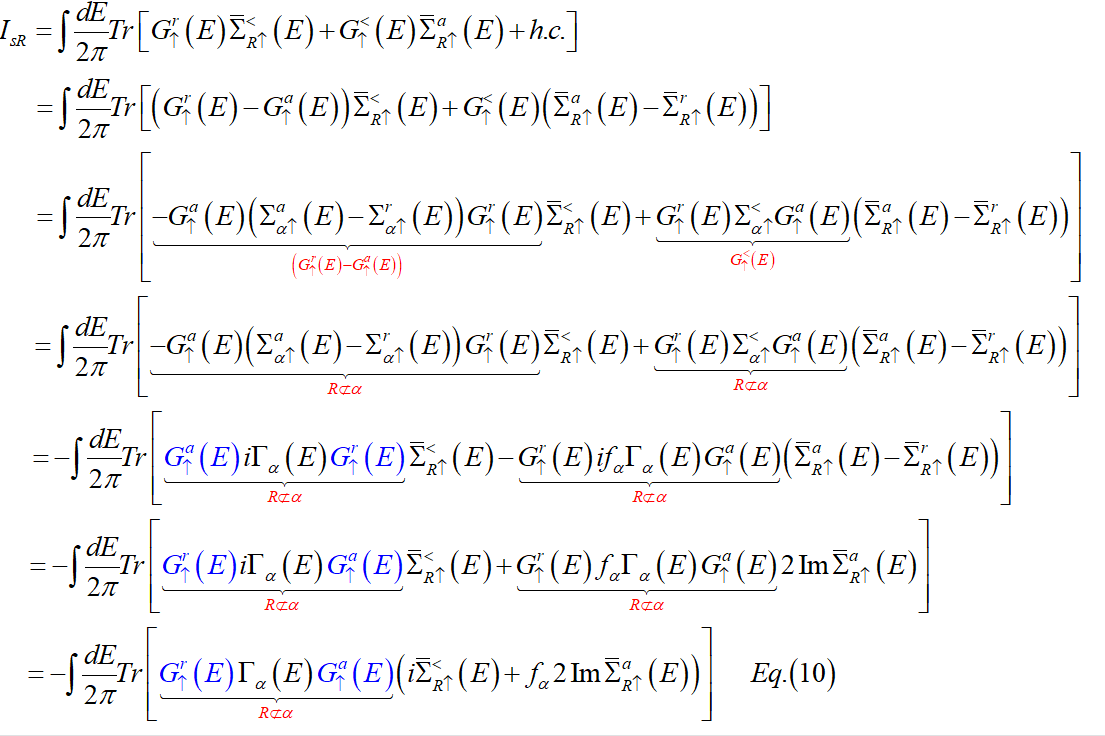
\includegraphics[width=0.65\textwidth, height=0.5\textwidth]{figures/eq1.png}
\end{figure}
\subsection{Expand $I_{L\sigma}$ in order of $J_q^2$ }
Expanding our result and keeping in order of $J_q^2$, it should give results of [\onlinecite{Ren}] and [\onlinecite{Wu}]. Keep 2-nd order in Dyson's equation, we have
\begin{gather}
G^r_{d\uparrow} =G^r_{L\uparrow} + G^r_{L\uparrow} {\bar \Sigma}^r G^r_{d\uparrow} = 1/[(G^r_{L\uparrow})^{-1} - {\bar \Sigma}^r] \simeq G^r_{L\uparrow} + G^r_{L\uparrow} {\bar \Sigma}^r G^r_{L\uparrow} ,\\
G^a_{d\uparrow} =G^a_{L\uparrow} + G^a_{L\uparrow} {\bar \Sigma}^a G^a_{d\uparrow} \simeq G^a_{L\uparrow} + G^a_{L\uparrow} {\bar \Sigma}^a G^a_{L\uparrow} , \\
G^r_{d\uparrow} - G^a_{d\uparrow} \simeq G^r_{L\uparrow} + G^r_{L\uparrow} {\bar \Sigma}^r G^r_{L\uparrow} - G^a_{L\uparrow} - G^a_{L\uparrow} {\bar \Sigma}^a G^a_{L\uparrow}
\end{gather}
\begin{gather}
\begin{split}
 G^<_{d\uparrow} &=  G^r_{d\uparrow} ( {\Sigma_{L\sigma}^{<} + \bar \Sigma}^<) G^a_{d\uparrow} \simeq [G^r_{L\uparrow} + G^r_{L\uparrow} {\bar \Sigma}^r G^r_{L\uparrow}] ( {\Sigma_{L\sigma}^{<} + \bar \Sigma}^<) [G^a_{L\uparrow} + G^a_{L\uparrow} {\bar \Sigma}^a G^a_{L\uparrow}] \\
& \simeq (G^r_{L\uparrow} \bar\Sigma^{<} + G^r_{L\uparrow} {\bar \Sigma}^r G^r_{L\uparrow}\Sigma_{L\sigma}^{<})G^a_{L\uparrow} + G^r_{L\uparrow} \Sigma_{L\sigma}^{<} G^a_{L\uparrow} {\bar \Sigma}^a G^a_{L\uparrow} \\
&\simeq (G^r_{L\uparrow} \bar\Sigma^{<} + G^r_{L\uparrow} {\bar \Sigma}^r G^r_{L\uparrow}\Sigma_{L\sigma}^{<} + G^r_{L\uparrow} \Sigma_{L\sigma}^{<} G^a_{L\uparrow} {\bar \Sigma}^a )G^a_{L\uparrow} \\
&\simeq G^r_{L\uparrow}( \bar\Sigma^{<} +  {\bar \Sigma}^r G^r_{L\uparrow}\Sigma_{L\sigma}^{<} + \Sigma_{L\sigma}^{<} G^a_{L\uparrow} {\bar \Sigma}^a )G^a_{L\uparrow}
\end{split}
\end{gather}
Then,
\begin{equation}
\begin{split}
I_\uparrow =&\int dE {\rm Tr} [(G_{d\uparrow}^r(E)-G_{d\uparrow}^a(E))\Sigma^<_{L\uparrow}(E) +G_{d\uparrow}^<(E) (\Sigma_{L\uparrow}^a(E) -\Sigma_{L\uparrow}^r(E))] \\
\simeq&\int dE {\rm Tr} [(G^r_{L\uparrow} + G^r_{L\uparrow} {\bar \Sigma}^r G^r_{L\uparrow} - G^a_{L\uparrow} - G^a_{L\uparrow} {\bar \Sigma}^a G^a_{L\uparrow})\Sigma_{L\sigma}^{<} + G^r_{L\uparrow}( \bar\Sigma^{<} +  {\bar \Sigma}^r G^r_{L\uparrow}\Sigma_{L\sigma}^{<} + \Sigma_{L\sigma}^{<} G^a_{L\uparrow} {\bar \Sigma}^a )G^a_{L\uparrow} (\Sigma_{L\sigma}^{a}-\Sigma_{L\sigma}^{r})] \\
\simeq& [(G^r_{L\uparrow} + G^r_{L\uparrow} {\bar \Sigma}^r G^r_{L\uparrow} - G^a_{L\uparrow} - G^a_{L\uparrow} {\bar \Sigma}^a G^a_{L\uparrow})if_{L\sigma}\Gamma_{L\sigma} + G^r_{L\uparrow}( \bar\Sigma^{<} +  {\bar \Sigma}^r G^r_{L\uparrow}\Sigma_{L\sigma}^{<} + \Sigma_{L\sigma}^{<} G^a_{L\uparrow} {\bar \Sigma}^a )G^a_{L\uparrow} (-\Gamma_{L\sigma})] \\
\simeq& [if_{L\sigma}G^r_{L\uparrow} + if_{L\sigma}G^r_{L\uparrow} {\bar \Sigma}^r G^r_{L\uparrow} - if_{L\sigma}G^a_{L\uparrow} - if_{L\sigma}G^a_{L\uparrow} {\bar \Sigma}^a G^a_{L\uparrow} - G^r_{L\uparrow}( \bar\Sigma^{<} +  {\bar \Sigma}^r G^r_{L\uparrow}\Sigma_{L\sigma}^{<} + \Sigma_{L\sigma}^{<} G^a_{L\uparrow} {\bar \Sigma}^a )G^a_{L\uparrow}] \Gamma_{L\sigma}
\end{split}
\end{equation}
or
\begin{eqnarray}
I_\uparrow = -\int d\omega \rho_R(\omega) (f^B_R(\omega)-f^B_L(\omega))\int dE (f_{L\uparrow}(E)-f_{L\downarrow}(E+\omega)) {\rm Tr}[A(E,\omega)] ,
\end{eqnarray}
where
\begin{equation}
\begin{split}
A(E,\omega)=&G^r_{d\uparrow} (D_{L\downarrow} \Gamma_{Rq}) G^a_{d\uparrow}\Gamma_{L\uparrow} .\\
\simeq&G^r_{L\uparrow}(D_{L\downarrow} \Gamma_{Rq}) G^a_{L\uparrow} 
 \end{split}
\end{equation}
In [\onlinecite{Ren}], Eq.~(2) gives
\begin{gather}
I_S=\frac{2 S_0}{\hbar} \int_0^{\infty} d \omega F_R(\omega) \int_{-\infty}^{\infty} d \varepsilon \rho_L(\varepsilon) \mathcal{W}(\varepsilon, \omega), \\ 
\mathcal{W}(\varepsilon, \omega)=  f_{L \downarrow}(\varepsilon+\hbar \omega)\left[1-f_{L \uparrow}(\varepsilon)\right]\left[1+N_R(\hbar \omega)\right]  -f_{L \uparrow}(\varepsilon)\left[1-f_{L \downarrow}(\varepsilon+\hbar \omega)\right] N_R(\hbar \omega)\\ \nonumber
=(f_{L\uparrow}-f_{L\downarrow})f_{L}^B(1+f_R) - f_{L\uparrow}f_R +f_{L\uparrow}f_{L\downarrow}f_R \\ \nonumber
=(f_{L\uparrow}-f_{L\downarrow})f_{L}^B + (f_{L\uparrow}-f_{L\downarrow})f_{L}^Bf_R - f_{L\uparrow}f_R +f_{L\uparrow}f_{L\downarrow}f_R \\ \nonumber
=(f_{L\uparrow}-f_{L\downarrow})f_{L}^B + (f_{L\uparrow}f_{L}^B - f_{L\downarrow} f_{L}^B - f_{L\uparrow} +f_{L\uparrow}f_{L\downarrow})f_R \\ \nonumber
=(f_{L\uparrow}-f_{L\downarrow})f_{L}^B + (-f_{L\uparrow}f_{L\downarrow}+f_{L\downarrow} - f_{L\uparrow} +f_{L\uparrow}f_{L\downarrow})f_R \\ \nonumber
= (f_{L\uparrow}-f_{L\downarrow})f_{L}^B + (f_{L\downarrow} - f_{L\uparrow})f_R \\
= (f_{L\uparrow}-f_{L\downarrow})(f_{L}^B - f_R )
\end{gather}
Spin-down current is given by
\begin{eqnarray}
I_{\downarrow} = \int dE [(G_{d\downarrow}^>-G_{d\downarrow}^< )\Sigma_{L\downarrow}^< +G_{d\downarrow}^< (\Sigma_{L\downarrow}^a-\Sigma_{L\downarrow}^r)]&&=-\int dE \sum_q [(f_{L\downarrow}-f_{L\uparrow})f_R+(f_{L\downarrow}-1)f_{L\uparrow}]\nonumber\\
&&\times G^r_{d\downarrow} (D_{L\uparrow} \Gamma_{Rq}) G^a_{d\downarrow}\Gamma_{L\downarrow} \nonumber
\end{eqnarray}
\subsection{Linear response regime}
\begin{equation}\label{eq:fupdown0}
\begin{split}
f_{R}(\omega)-f_{L}^{B}(\omega) &= \frac{1}{e^{\beta_{R}\omega}-1} - \frac{1}{e^{\beta_{L}(\omega+\Delta\mu_{s})}-1} \\
&= \frac{e^{\beta_{L}(\omega+\Delta\mu_{s})} - e^{\beta_{R}\omega}}{[e^{\beta_{R}\omega}-1][e^{\beta_{L}(\omega+\Delta\mu_{s})}-1]} \\
&= \frac{e^{\beta_{L}\omega}[e^{\beta_{L}\Delta\mu_{s}} - e^{(\beta_{R}-\beta_{L})\omega}]}{e^{\beta_{L}\omega}[e^{(\beta_{R}-\beta_{L})\omega}-e^{-\beta_{L}\omega}][e^{\beta_{L}(\omega+\Delta\mu_{s})}-1]} \\
&= \frac{e^{\beta_{L}\Delta\mu_{s}} - e^{(\beta_{R}-\beta_{L})\omega}}{[e^{(\beta_{R}-\beta_{L})\omega}-e^{-\beta_{L}\omega}][e^{\beta_{L}(\omega+\Delta\mu_{s})}-1]}.
\end{split}
\end{equation}
\begin{equation}
\begin{split}
f_{L\uparrow}(E)-f_{L\downarrow}(E+\omega) &= \frac{1}{e^{\beta_{L}(E-\mu_{L\uparrow})}+1} - \frac{1}{e^{\beta_{L}(E+\omega-\mu_{L\downarrow})}+1}.
\end{split}
\end{equation}
Here $\Delta\mu_{s} = \mu_{L\uparrow} - \mu_{L\downarrow}$ as before, and $\beta_{R}-\beta_L = \frac{\Delta T}{k_{B}T_{L}T_{R}}$. 
\subsubsection{$\Delta\mu_s=0$ and $\Delta T\to 0$ limit}
If $\Delta\mu_{s} = 0$, we have
\begin{equation}
\begin{split}
f_{R}(\omega)-f_{L}^{B}(\omega) & =\frac{e^{\beta_{L}\Delta\mu_{s}} - e^{(\beta_{R}-\beta_{L})\omega}}{[e^{(\beta_{R}-\beta_{L})\omega}-e^{-\beta_{L}\omega}][e^{\beta_{L}(\omega+\Delta\mu_{s})}-1]} \\
&\stackrel{\Delta \mu_s= 0}{\rightarrow} \frac{1-e^{(\beta_{R}-\beta_{L})\omega}}{[e^{(\beta_{R}-\beta_{L})\omega}-e^{-\beta_{L}\omega}][e^{\beta_{L}\omega}-1]}
\end{split}
\end{equation}

\begin{equation}\label{eq:fupdown}
\begin{split}
f_{L\uparrow}(E)-f_{L\downarrow}(E+\omega) &= \frac{1}{e^{\beta_{L}(E-\mu_{L})}+1} - \frac{1}{e^{\beta_{L}(E+\omega-\mu_{L})}+1}.
\end{split}
\end{equation}
In $\Delta T\to 0$ limit, $\beta_{R}-\beta_{L} \to 0$,
\begin{equation}
e^{(\beta_{R}-\beta_{L})\omega} = 1 + \omega\beta_{L}^{2} k_{B}\Delta T + O(\Delta T^{2}),
\end{equation}
then,
\begin{equation}
\begin{split}
f_{R}(\omega)-f_{L}^{B}(\omega) &\stackrel{\Delta T\to 0}{\rightarrow}  \frac{\omega k_{B}\beta_{L}^{2} } {[ 1 - e^{-\beta_{L}\omega}] [1-e^{\beta_{L} \omega}]}\Delta T \\
& \stackrel{\Delta T\to 0}{\rightarrow} \frac{-\omega k_{B}\beta_{L}^{2}} {4\rm{sinh}^2(\beta_{L}\omega/2)}\Delta T  = \frac{-\omega k_{B}\beta_{L}^{2}} {2[\rm{cosh}(\beta_{L}\omega)-1]}\Delta T.
\end{split}
\end{equation}
Note that
\[
\rm{sinh}^2(\frac{x}{2}) = \frac{1}{2}[\rm{cosh}(x)-1].
\]
\begin{equation}\label{eq:fupdown}
\begin{split}
f_{L\uparrow}(E)-f_{L\downarrow}(E+\omega) & \stackrel{\Delta T\to 0}{\rightarrow} 0.
\end{split}
\end{equation}
When $\omega=0$, the Eq.~(\ref{eq:fupdown}) is 0, thus the total coefficient is not singular. 
\subsubsection{$\Delta T=0$ limit, and $\Delta\mu_s\to0$}
When $\Delta T = 0$, $\beta_{R} - \beta_{L} = 0$. The Eq.~(\ref{eq:fupdown0}) reduces to
\begin{equation}
\begin{split}
f_{R}(\omega)-f_{L}^{B}(\omega) & =\frac{e^{\beta_{L}\Delta\mu_{s}} - e^{(\beta_{R}-\beta_{L})\omega}}{[e^{(\beta_{R}-\beta_{L})\omega}-e^{-\beta_{L}\omega}][e^{\beta_{L}(\omega+\Delta\mu_{s})}-1]} \\
&\stackrel{\Delta T= 0}{\rightarrow} \frac{e^{\beta_{L}\Delta\mu_{s}} - 1}{ [1 - e^{-\beta_{L}\omega}][e^{\beta_{L}(\omega+\Delta\mu_{s})}-1]}\\
&\stackrel{\Delta \mu_s\to 0}{\rightarrow} \frac{e^{\beta_{L}\Delta\mu_{s}} - 1}{ [1 - e^{-\beta_{L}\omega}][e^{\beta_{L}\omega}-1]} \\
&\stackrel{\Delta \mu_s\to 0}{\rightarrow} \frac{-\beta_{L}\Delta\mu_{s}}{ [1 - e^{-\beta_{L}\omega}][1-e^{\beta_{L}\omega}]} \\
& \stackrel{\Delta \mu_s\to 0}{\rightarrow} \frac{\beta_{L}} {4\rm{sinh}^2(\beta_{L}\omega/2)} \Delta\mu_{s}= \frac{\beta_{L}} {2[\rm{cosh}(\beta_{L}\omega)-1]}\Delta\mu_{s}.
\end{split}
\end{equation}
\begin{equation}
\begin{split}
f_{L\uparrow}(E)-f_{L\downarrow}(E+\omega) &= \frac{1}{e^{\beta_{L}(E-\mu_{L\uparrow})}+1} - \frac{1}{e^{\beta_{L}(E+\omega-\mu_{L\downarrow})}+1} \\
&= \frac{e^{\beta_{L}(E+\omega-\mu_{L\downarrow})}- e^{\beta_{L}(E-\mu_{L\uparrow})}} {[e^{\beta_{L}(E-\mu_{L\uparrow})}+1] [e^{\beta_{L}(E+\omega-\mu_{L\downarrow})}+1]} \\
& = \frac{e^{\beta_L(E-\mu_{L\uparrow})} [e^{\beta_{L}(\omega+\Delta\mu_s)}- 1]} {[e^{\beta_{L}(E-\mu_{L\uparrow})}+1] e^{\beta_L(E-\mu_{L\uparrow})} [e^{\beta_{L}(\omega+\Delta\mu_s)}+e^{-\beta_L(E-\mu_{L\uparrow})}]}
\end{split}
\end{equation}
\subsubsection{linear response regime}
In summary, we have
\begin{equation}
\begin{split}
f_{R}(\omega)-f_{L}^{B}(\omega) &= \frac{-\omega k_B\beta^2\Delta T + \beta\Delta\mu_s}{2[\rm{cosh}(\beta_{L}\omega)-1]}
\end{split}
\end{equation}
Additionally, when $\omega\to0$,
\[
\lim_{\omega\to0}\omega f_{R}(\omega) = \frac{\omega}{e^{\beta_{R}\omega}-1} = \frac{1}{\beta_R}.
\]
(1) For $\Delta\mu_s=0$, when $\omega\to0$,
\[
\lim_{\omega\to0}\omega f_{L}^{B}(\omega) = \frac{\omega}{e^{\beta_{L}(\omega+\Delta\mu_{s})}-1} = \frac{1}{\beta_L}.
\]
Then for $\Delta\mu_s=0$ and limits $\Delta T\to 0$, $\omega\to 0$,
\begin{equation}
\begin{split}
\omega[f_{R}(\omega)-f_{L}^{B}(\omega)] &= \frac{1}{\beta_R} - \frac{1}{\beta_L} \\
& = -k_B \Delta T.
\end{split}
\end{equation}
(2) For $\Delta T=0$, when $\omega\to0$ and $\Delta\mu_s\to 0$,
\[
\lim_{\omega\to0}\omega f_{L}^{B}(\omega) = \frac{\omega}{e^{\beta_{L}(\omega+\Delta\mu_{s})}-1} = \frac{1}{\beta_L e^{\beta_L \Delta\mu_s}}.
\]
Then for $\Delta T=0$ and limits $\Delta \mu_s\to 0$, $\omega\to 0$,
\begin{equation}
\begin{split}
\omega[f_{R}(\omega)-f_{L}^{B}(\omega)] &= \frac{1}{\beta_R} - \frac{1}{\beta_Le^{\beta_L \Delta\mu_s}} 
\end{split}
\end{equation}

\subsection{Ways to reduce time-consuming}
\subsubsection{Low temperature}
In transport problem, the Landauer type formula has term of the difference of two Fermionic distribution. Generally, this constrains the range of integrating variable to $[-\frac{T}{2}, \frac{T}{2}]$ or $[\mu_{1}, \mu_{2}]$.
\subsubsection{Physical consideration}
Usually, only several subbands or transverse modes are investigated, which suggests the integrating range of $[-\frac{T}{2}, E_{i+1}]$ to include i subbands, with $E_i$ the $i$th subband energy threshold. When integrating a very high energy, 
\subsubsection{Repalcing repeating calculations by interpolation}
If a complex manipulation, like matrix inverse, is contained in a loop,
we can take the matrix inverse out of loop, and replace it with an interpolation of inversed matrice calculated earlier. Interpolating by
\begin{equation}
f(c) = \frac{f(a) - f(b)}{a-b}\times (c-a) + f(a).
\end{equation}
\subsubsection{$Tr[\Gamma_{Rq}'D_{L\uparrow}(E)D_{L\downarrow}(E+\omega)\Gamma_{Rq}']$}
$\Gamma_{Rq}'$ is block matrix of dimension  $n_{wid}n_{len}\times n_{wid}n_{len}$, with only $I_{n_{wid}\times n_{wid}}$ block. For n\_wid=3, n\_len=5, we have
\begin{equation}
\Gamma_{L}' = \left[\begin{array}{cccc}
\Gamma_{3\times 3}^{L} & 0 & 0 & 0 \\
0 & 0 & 0 & 0 \\
0 & 0 & 0 & 0 \\
0 & 0 & 0 & 0
\end{array}\right],
\end{equation}
\begin{equation}
\Gamma_{Rq}' = \left[\begin{array}{cccc}
0 & 0 & 0 & 0 \\
0 & 0 & 0 & 0 \\
0 & 0 & 0 & 0 \\
0 & 0 & 0 & I_{3\times 3}
\end{array}\right].
\end{equation}
\begin{equation}
D_{L\uparrow} = G_{L\uparrow}^{r}\Gamma_{L\uparrow}G_{L\uparrow}^{a} = 
\left[\begin{array}{cccc}
G_{11}^{r}\Gamma_{3\times3}^{L} & 0 & 0 & 0 \\
G_{21}^{r}\Gamma_{3\times3}^{L} & 0 & 0 & 0 \\
G_{31}^{r}\Gamma_{3\times3}^{L} & 0 & 0 & 0 \\
G_{41}^{r}\Gamma_{3\times3}^{L} & 0 & 0 & 0 \\
\end{array}\right]
\left[\begin{array}{cccc}
G_{11}^{a} & G_{12}^{a} & G_{13}^{a} & G_{14}^{a} \\
G_{21}^{a} & G_{22}^{a} & G_{23}^{a} & G_{24}^{a} \\
G_{31}^{a} & G_{32}^{a} & G_{33}^{a} & G_{34}^{a} \\
G_{41}^{a} & G_{42}^{a} & G_{43}^{a} & G_{44}^{a} \\
\end{array}\right].
\end{equation}
Then,
\begin{equation}
\begin{split}
\Gamma_{Rq}'D_{L\uparrow} = 
\left[\begin{array}{cccc}
0 & 0 & 0 & 0 \\
0 & 0 & 0 & 0 \\
0 & 0 & 0 & 0 \\
\rm{x} & \rm{x} & \rm{x} & \rm{x}
\end{array}\right]
&= \left[\begin{array}{cccc}
0 & 0 & 0 & 0 \\
0 & 0 & 0 & 0 \\
0 & 0 & 0 & 0 \\
G_{41}^{r}\Gamma_{3\times3}^{L}G_{11}^{a} & G_{41}^{r}\Gamma_{3\times3}^{L}G_{12}^{a} & G_{41}^{r}\Gamma_{3\times3}^{L}G_{13}^{a} & G_{41}^{r}\Gamma_{3\times3}^{L}G_{14}^{a} \\
\end{array}\right]
\end{split}
\end{equation}
and
\begin{equation}
D_{L\downarrow}\Gamma_{Rq}' = 
\left[\begin{array}{cccc}
0 & 0 & 0 & \rm{x} \\
0 & 0 & 0 & \rm{x} \\
0 & 0 & 0 & \rm{x} \\
0 & 0 & 0 & \rm{x}
\end{array}\right] = 
\left[\begin{array}{cccc}
0 & 0 & 0 & G_{11}^{r}\Gamma_{3\times3}^{L}G_{14}^{a}\\
0 & 0 & 0 & G_{21}^{r}\Gamma_{3\times3}^{L}G_{14}^{a} \\
0 & 0 & 0 & G_{31}^{r}\Gamma_{3\times3}^{L}G_{14}^{a} \\
0 & 0 & 0 & G_{41}^{r}\Gamma_{3\times3}^{L}G_{14}^{a} \\
\end{array}\right]
\end{equation}
So 
\begin{equation}
\Gamma_{Rq}'D_{L\uparrow}D_{L\downarrow}\Gamma_{Rq}' = 
\left[\begin{array}{cccc}
0 & 0 & 0 & 0 \\
0 & 0 & 0 & 0 \\
0 & 0 & 0 & 0 \\
0 & 0 & 0 & A(E,\omega)
\end{array}\right].
\end{equation}
\begin{equation}
[A(E, \omega)]_{ij} = G_{41}^{r}\Gamma_{3\times3}^{L}G_{1i}^{a} G_{j1}^{r}\Gamma_{3\times3}^{L}G_{14}^{a},
\end{equation}
the advanced Green's function is related to the retarded Green's function by
\begin{equation}
G^{a} = [G^{r}]^{\dag},
\end{equation}
which gives
\begin{equation}
[A(E, \omega)]_{ij} = G_{41}^{r}\Gamma_{3\times3}^{L}[G^{r}]_{1i}^{\dag} G^{r}_{j1}\Gamma_{3\times3}^{L}[G^{r}]_{14}^{\dag}.
\end{equation}
Here $G_{ij}^{r}$ is a $3\times 3$ matrix in full matrix G$^{r}$ of dimension $12\times12$, and $\{i, j\}\in [1,2,3,4]$.
\begin{equation}
Tr[A(E, \omega)] = \sum_{i}G_{41}^{r}\Gamma_{3\times3}^{L}[G^{r}]_{1i}^{\dag} G^{r}_{i1}\Gamma_{3\times3}^{L}[G^{r}]_{14}^{\dag}.
\end{equation}

\subsubsection{interpolate on $Tr[A(E,\omega)$]}

\begin{figure}
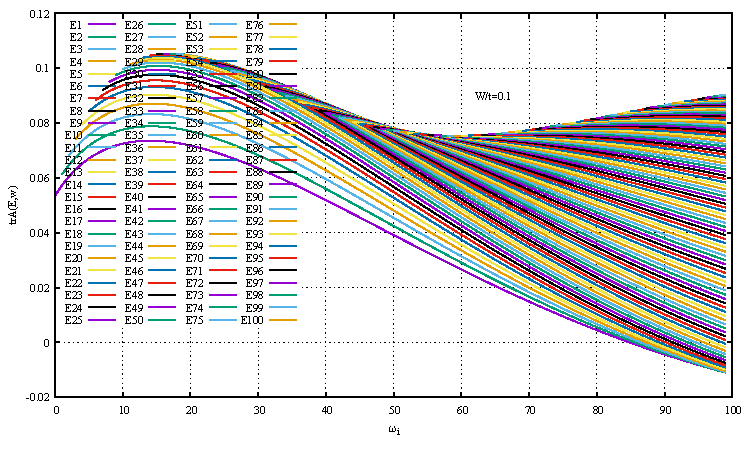
\includegraphics[width=8.5cm]{figures/trA.pdf}
\caption{\label{fig:trA} $TrA$ for the clean NM-NM-FI system.}
\end{figure}

The interpolation to $trA$ reduces computation from 10000 points to 1000 points.



\section{Spin current in altermagnetic metal/altermagnetic metal/ferromagnetic insulator system}
\subsection{Hamiltonian of a two-terminal AM/AM/FI system}
For system consists of an altermagnetic metal (AM) region sandwiched by a left AM lead and a right ferromagnetic insulating (FI) lead, the Hamiltonian is
\begin{align}
H&=H_{\rm L}+H_{\rm C}+H_{\rm R}+H_{\rm T}+H_{\rm sd},
\end{align}
in which, the left lead and the central region is described by
\begin{equation}\label{eq:He}
H_{e}(\mathbf{k})= tk^2 + 2t_J k_x k_y \sigma_z.
\end{equation}
Then we have
\begin{align}
H_{\rm{L}} &= \sum_{k\sigma} \epsilon_{\sigma}(k) c_{k\sigma}^{\dag} c_{k\sigma},\\
H_{\rm{C}} &= \sum_{n\sigma}\varepsilon_{n\sigma} d_{n\sigma}^{\dagger} d_{n\sigma},\\
H_{\rm{R}} &\approx \sum_{q} \hbar w_{q} a_{q}^{\dagger} a_{q},
\end{align}
are Hamiltonians of left lead, central region and right lead respectively. The electron dispersion $\epsilon_{\sigma}(k)= tk^2+2\sigma t_Jk_xk_y$, with $\sigma=\pm 1$ for spin-$\uparrow$ and spin-$\downarrow$. $H_{\rm T}$ is the hopping between the left lead and the central region, while $H_{\rm sd}$ is the exchange coupling between right lead and central region,
\begin{align}
H_{\rm{T}} =& \sum_{nk\sigma}( t_{nk\sigma} c_{k \sigma}^{\dagger} d_{n\sigma} + t_{nk\sigma}^{*} d_{n\sigma}^{\dagger} c_{k\sigma}),\\
H_{\rm{sd}}=& -\sum_{q n n^{\prime}} J_{q n n^{\prime}} a_q^{\dagger} d_{n \uparrow}^{\dag} d_{n^{\prime} \downarrow} +\text { h.c. }
\end{align}

\subsection{DC spin current of a two-terminal AM/AM/FI system}

Since the system Hamiltonian $H$ remains unchanged, the spin current formulas in this system is the same as those in NM/NM/FI system. Left lead electron currents in a two-terminal NM/FI system were
\begin{eqnarray}
I_{\uparrow} &&= \int \frac{dE}{2\pi} {\rm Tr} [(G_{\uparrow}^r(E)-G_{\uparrow}^a(E))\Sigma^<_{L\uparrow}(E)+G_{\uparrow}^<(E) (\Sigma_{L\uparrow}^a(E) -\Sigma_{L\uparrow}^r(E))],\\
I_{\downarrow} &&= \int \frac{dE}{2\pi} {\rm Tr} [(G_{\downarrow}^r(E)-G_{\downarrow}^a(E))\Sigma^<_{L\downarrow}(E)+G_{\downarrow}^<(E) (\Sigma_{L\downarrow}^a(E) -\Sigma_{L\downarrow}^r(E))].
\end{eqnarray}
In above equations, 
\begin{eqnarray}
G^r_{\sigma} =g^r_{d\sigma} + g^r_{d\sigma} \Sigma_{\sigma}^r G^r_{\sigma} = 1/[(g^r_{d\sigma})^{-1} - \Sigma_{\sigma}^r],
\end{eqnarray}
with $\Sigma_{\sigma}^r = \Sigma_{L\sigma}^r +  {\bar \Sigma}_{R\sigma}^r$ and
\begin{eqnarray}
{\bar \Sigma}^<_{R\uparrow}(E) &= \int d\omega ~ G^r_{L\downarrow}({E+\omega})[i \Gamma_{L\downarrow}({E+\omega}) f_{L\downarrow}({E+\omega})] G^a_{L\downarrow}({E+\omega})(1+f_R^B(\omega)) \Gamma_R(\omega),\label{eq:less} \\
{\bar \Sigma}^r_{R\uparrow}(E)&= \int d\omega G^r_{L\downarrow}({E+\omega})[f^B_R(\omega)-\Gamma_{L\downarrow}({E+\omega}) f_{L\downarrow}({E+\omega})G^a_{\downarrow}({E+\omega})(i/2)]\Gamma_R(\omega).\label{eq:rup}
\end{eqnarray}
\begin{eqnarray}
{\bar \Sigma}^<_{R\downarrow}(E) &= \int d\omega ~ G^r_{L\uparrow}({E-\omega})[i \Gamma_{L\uparrow}({E-\omega}) f_{L\uparrow}({E-\omega})] G^a_{L\uparrow}({E-\omega})(1+f_R^B(\omega)) \Gamma_R(\omega),\label{eq:less} \\
{\bar \Sigma}^r_{R\downarrow}(E)&= \int d\omega G^r_{L\uparrow}({E-\omega})[f^B_R(\omega)-\Gamma_{L\uparrow}({E-\omega}) f_{L\uparrow}({E-\omega})G^a_{\uparrow}({E-\omega})(i/2)]\Gamma_R(\omega).\label{eq:rdn}
\end{eqnarray}
Spin current from the right FI lead
\begin{eqnarray}
I_R^s &&= \int \frac{dE}{R\pi} {\rm Tr} [(G_{\uparrow}^r(E)-G_{\uparrow}^a(E))\bar\Sigma^<_{R\uparrow}(E)+G_{\uparrow}^<(E) (\bar\Sigma_{R\uparrow}^a(E) -\bar\Sigma_{R\uparrow}^r(E))].
\end{eqnarray}

\subsection{DC spin current expression in four-terminal AM/FI system}
Similarly, the electron current flowing out of metallic lead-$\alpha$ ($\alpha=1, 3, 4$) is given by
\begin{eqnarray}
I_{\alpha\uparrow} &&= \int \frac{dE}{2\pi} {\rm Tr} [(G_{\uparrow}^r(E)-G_{\uparrow}^a(E))\Sigma^<_{\alpha\uparrow}(E)+G_{\uparrow}^<(E) (\Sigma_{\alpha\uparrow}^a(E) -\Sigma_{\alpha\uparrow}^r(E))],\\
I_{\alpha\downarrow} &&= \int \frac{dE}{2\pi} {\rm Tr} [(G_{\downarrow}^r(E)-G_{\downarrow}^a(E))\Sigma^<_{\alpha\downarrow}(E)+G_{\downarrow}^<(E) (\Sigma_{\alpha\downarrow}^a(E) -\Sigma_{\alpha\downarrow}^r(E))].
\end{eqnarray}
In above equations, 
\begin{eqnarray}
G^r_{\sigma} =g^r_{d\sigma} + g^r_{d\sigma} \Sigma_{\sigma}^r G^r_{\sigma} = 1/[(g^r_{d\sigma})^{-1} - \Sigma_{\sigma}^r],
\end{eqnarray}
with $\Sigma_{\sigma}^r = \Sigma_{1\sigma}^r + \Sigma_{3\sigma}^r  + \Sigma_{4\sigma}^r + {\bar \Sigma}_{2\sigma}^r=\Sigma_{{\rm M}\sigma}^r+\bar\Sigma_{2\sigma}^r$. In BA, we have
\begin{eqnarray}
{\bar \Sigma}^<_{2\sigma}(E) &= \int d\omega ~ G^r_{{\rm M}\bar\sigma}({\bar E})[\sum_{\alpha\neq 2} i \Gamma_{\alpha\bar\sigma}({\bar E}) f_{\alpha\bar\sigma}({\bar E})] G^a_{{\rm M}\bar\sigma}({\bar E})(1+f_2^B(\omega)) \Gamma_2(\omega),\label{eq:less} \\
{\bar \Sigma}^r_{2\sigma}(E)&= \int d\omega G^r_{{\rm M}\bar\sigma}({\bar E})[f^B_2(\omega)-\sum_{\alpha\neq 2}\Gamma_{\alpha\bar\sigma}({\bar E}) f_{\alpha\bar\sigma}({\bar E})]G^a_{{\rm M}\bar\sigma}({\bar E})(i/2)\Gamma_2(\omega).\label{eq:r}
\end{eqnarray}
% \begin{eqnarray}
% {\bar \Sigma}^<_{2\sigma}(E) = i\int d\omega ~ (1+f_2^B(\omega)) f_{M\bar\sigma}({\bar E}) D^0_{M\bar\sigma}({\bar E})\Gamma_2(\omega) \label{sig1} \\
% {\bar \Sigma}^r_{2\sigma}(E)
% %=i \int \frac{d\omega}{2\pi} [G^r_{L\downarrow}({\bar E}) \Sigma_R^<(\omega)
% %+  G^<_{L\downarrow}({\bar E}){ \Sigma}^a_{R}(\omega)] \nonumber\\
% =\int d\omega [f_2(\omega) G^r_{M\bar\sigma}({\bar E})
% + i f_{M\bar\sigma}({\bar E}){\rm Im}G^r_{M\bar\sigma}({\bar E})]\Gamma_2,
% \end{eqnarray}
Here $\bar E=E-\sigma \omega$. $G_{M\sigma}^r=1/[(g^r_{d\sigma})^{-1} - \Sigma_{{\rm M}\sigma}^r]$ is the Green's function of the central region with the three metallic leads only. For SCBA, the corresponding extrpolation is $G_{{\rm M}\sigma}^r \to G_{\sigma}^r$ and adding $\Sigma_2^{r,<}$ in summation $\sum_{\alpha}$.

\textcolor{red}{Note Hamiltonian (\ref{eq:He}) is not in pseudo-spin space, $\sigma_z$ labels the true spin-space, therefore the spin degree of freedom is spit. $G_{\uparrow}$, $G_{\downarrow}$ and $\Sigma_{\alpha\uparrow}$, $\Sigma_{\alpha\downarrow}$ even $g_{d\uparrow}$ and $g_{d\downarrow}$ are no longer degenerate. For a spin-diagonal Hamiltonian (\ref{eq:He}), we can calculate the Green's function of spin-$\sigma$ Hamiltonian seperately.} The GF of central region with $H_{C\sigma}$ is
\begin{eqnarray}
g_{d\sigma}^r = 1/[E-H_{C\sigma}],
\end{eqnarray}
where $H_{C\sigma}$ is the submatrix of $H_{C}$ is spin-space representation. %See derivation of Eqs.~(\ref{eq:less}) and (\ref{eq:r}) in Appendix.

{\noindent \textbf{\textit{Check current conservation}}} -- Considering the continuity equity of electron current and spin current, we should have
\begin{gather}
\sum_{\alpha=1,3,4}I_{\alpha\uparrow} + \sum_{\alpha=1,3,4}I_{\alpha\downarrow} = 0,\\
\sum_{\alpha=1,2,3,4}I_{\alpha}^s = 0.
\end{gather}

Now we check these conditions. \textcolor{red}{The energy spectrum of up spin and down are degenerate, need extra shift? In implementation, energy integration range: $[\mu_1-10T, \mu_1+10T]$.} Obviously, $\sum_{\alpha=1,3,4}I_{\alpha\sigma}\neq 0$.
\begin{gather}
\begin{split}
\sum_{\alpha=1,3,4}I_{\alpha\uparrow} &= \int \frac{dE}{2\pi} {\rm Tr} [(G_{\uparrow}^r(E)-G_{\uparrow}^a(E))\sum_{\alpha=1,3,4} \Sigma^<_{\alpha\uparrow}(E) + G_{\uparrow}^<(E) \sum_{\alpha=1,3,4}(\Sigma_{\alpha\uparrow}^a(E) -\Sigma_{\alpha\uparrow}^r(E))],\\
& = \int \frac{dE}{2\pi} {\rm Tr} [(G_{\uparrow}^r(E)-G_{\uparrow}^a(E))\sum_{\alpha=1,3,4} if_{\alpha\uparrow}(E)\Gamma_{\alpha\uparrow}(E) + G_{\uparrow}^<(E) \sum_{\alpha=1,3,4}i\Gamma_{\alpha\uparrow}(E)] \\
\end{split}
\end{gather}
Similarly, we have
\begin{gather}
\begin{split}
\sum_{\alpha=1,3,4}I_{\alpha\downarrow} &= \int \frac{dE}{2\pi} {\rm Tr} [(G_{\downarrow}^r(E)-G_{\downarrow}^a(E))\sum_{\alpha=1,3,4} \Sigma^<_{\alpha\downarrow}(E) + G_{\downarrow}^<(E) \sum_{\alpha=1,3,4}(\Sigma_{\alpha\downarrow}^a(E) -\Sigma_{\alpha\downarrow}^r(E))]\\
&=\int \frac{dE}{2\pi} {\rm Tr} [(G_{\downarrow}^r(E)-G_{\downarrow}^a(E))\sum_{\alpha=1,3,4} if_{\alpha\downarrow}(E)\Gamma_{\alpha\downarrow}(E) + G_{\downarrow}^<(E) \sum_{\alpha=1,3,4}i\Gamma_{\alpha\downarrow}(E)]
\end{split}
\end{gather}
The leads are thermalized at the same temperatures and different chemical potentials, also $f_{\alpha\sigma}=f_{\alpha\bar\sigma}$ for three metallic leads. Taylor expansion gives
\begin{gather}
\begin{split}
f_{1\sigma}(E, V, T) &= f_0(E, V_0, T_0),\\
f_{3\sigma}(E, V, T) &= f_0(E, V_0+\delta V/2, T_0)=f_0+\frac{\delta V}{2} f'+\cdots,\\
f_{4\sigma}(E, V, T) &= f_0(E, V_0-\delta V/2, T_0)=f_0-\frac{\delta V}{2} f'+\cdots.
\end{split}
\end{gather}
The three AM leads are the same material,
\begin{gather}
\Gamma_{1\sigma} = \Gamma_{3\sigma}=\Gamma_{4\sigma}=\frac{1}{3}\Gamma_{{\rm M}\sigma},\\
\Sigma_{\alpha\sigma} \neq \Sigma_{\alpha\bar\sigma},\\
\Gamma_{\alpha\sigma} \neq \Gamma_{\alpha\bar\sigma}.
\end{gather}
Then, 
\begin{gather}
\begin{split}
\sum_{\alpha=1,3,4}I_{\alpha\uparrow} & = \int \frac{dE}{2\pi} {\rm Tr} [(G_{\uparrow}^r(E)-G_{\uparrow}^a(E))\frac{1}{3}\Gamma_{{\rm M}\uparrow}(E) \sum_{\alpha=1,3,4} if_{\alpha\uparrow}(E) + G_{\uparrow}^<(E) \times i\Gamma_{{\rm M}\uparrow}(E)], \\
\sum_{\alpha=1,3,4}I_{\alpha\downarrow} & = \int \frac{dE}{2\pi} {\rm Tr} [(G_{\downarrow}^r(E)-G_{\downarrow}^a(E))\frac{1}{3}\Gamma_{{\rm M}\downarrow}(E) \sum_{\alpha=1,3,4} if_{\alpha\downarrow}(E) + G_{\downarrow}^<(E) \times i\Gamma_{{\rm M}\downarrow}(E)].
\end{split}
\end{gather}
\begin{gather}
\begin{aligned}
\int\frac{dE}{2\pi} {\rm Tr}[ iG^{ >}\Gamma _{M\uparrow }( f_1+f_3+f_4) - iG^{ <}\Gamma _{M_{\uparrow }}( f_{1}+f_{3}+f_{4}+1)]
\end{aligned}
\end{gather}

\section{Formulas in PRB. 88, 220406(R) (2013)}
\subsection{Formula 1}
System Hamiltonion:
\begin{equation}
H=H_{L}+H_{R}+H_{s d}.
\end{equation}
Left lead is metallic
\begin{equation}
H_{L} = \sum_{k\sigma} \left(\varepsilon_{k\sigma}-\mu_{\sigma}\right) c_{k \sigma}^{\dagger} c_{k \sigma},
\end{equation}
right lead is insulating magnetic
\begin{equation}
H_{R} \approx \sum_{q} \hbar w_{q} a_{q}^{\dagger} a_{q}+\text { constant }.
\end{equation}
The interfacial electron-magnon interaction is described by
\begin{equation}
H_{s d}=-\sum_{k, q} J_{q}\left[S_{q}^{-} c_{k \uparrow}^{\dagger} c_{k+q \downarrow}+S_{q}^{+} c_{k+q \downarrow}^{\dagger} c_{k \uparrow}\right]
\end{equation}
where $S_{q}^{-} \approx \sqrt{2 S_{0}} a_{q}^{\dagger}, S_{q}^{+} \approx \sqrt{2 S_{0}} a_{q}$ are in the momentum space and $J_{q}$ denotes the effective exchange coupling at the interface. The magnonic spin current operator can be obtained by
\begin{equation}
\hat{I}_{S} = \frac{d\hat{N}_{R}}{dt} =  \frac{d}{dt} \sum_{q}a_{q}^{\dag}a_{q},
\end{equation}
the magnonic spin current is obtained by taking average over the nonequilibrium ground state $\ket{\psi_{0}}$ of the interacting system $H$:
\begin{equation}
I_{S} = \frac{dN_{R}}{dt} =  \frac{d}{dt} \langle \sum_{q}a_{q}^{\dag}a_{q}\rangle.
\end{equation}
Using the Heisenberg equation, we get
\begin{equation}
I_{S}=\frac{i}{\hbar}\langle[H_{s d}, \sum_{q} a_{q}^{\dagger} a_{q}]\rangle.
\end{equation}
\begin{equation}
[H_{s d}, \sum_{q} a_{q}^{\dagger} a_{q}] = [-\sum_{k, q} J_{q}\left(S_{q}^{-} c_{k \uparrow}^{\dagger} c_{k+q \downarrow}+S_{q}^{+} c_{k+q \downarrow}^{\dagger} c_{k \uparrow}\right), \sum_{q} a_{q}^{\dagger} a_{q}],
\end{equation}
in which,
\begin{equation}
[a_{q}^{\dag}, \sum_{q^{\prime}} a_{q'}^{\dagger} a_{q^{\prime}}] = \delta_{q q^{\prime}}[a_{q}^{\dagger}, a_{q^{\prime}}^{\dagger} a_{q^{\prime}}] = [a_{q}^{\dagger}, a_{q}^{\dagger} a_{q}] = a_{q}^{\dagger}[a_{q}^{\dagger}, a_{q}] = - a_{q}^{\dagger}.
\end{equation}
Similarly,
\begin{equation}
[a_{q}, \sum_{q^{\prime}} a_{q^{\prime}}^{+} a_{q^{\prime}}]=[a_{q}, a_{q}^{\dagger} a_{q}]=a_{q}.
\label{eq:1-1}
\end{equation}
So,
\begin{equation}
\begin{split}
I_{S} &=\frac{i}{\hbar}\langle -\sum_{k q} J_{q}\left(-S_{q}^{-} c_{k \uparrow}^{\dagger} c_{k+q\downarrow} + S_{q}^{+} c_{k+q\downarrow}^{\dagger} c_{k \uparrow}\right) \rangle \\
&= \frac{i}{\hbar} \sum_{k q} J_{q}\left( \langle S_{q}^{-} c_{k \uparrow}^{\dagger} c_{k+q\downarrow}\rangle - \langle S_{q}^{+} c_{k+q\downarrow}^{\dagger} c_{k \uparrow}\rangle \right).
\end{split}
\end{equation}
\subsection{Formula 2}
\begin{equation}
\frac{d}{d t}\left\langle S_{q}^{+} c_{k+q \downarrow}^{\dagger} c_{k \uparrow}\right\rangle=\frac{i}{\hbar}\left\langle\left[H_{L}+H_{s d}+H_{R}, S_{q}^{+} c_{k+q \downarrow}^{\dagger} c_{k \uparrow}\right]\right\rangle.
\label{eq:2-1}
\end{equation}
The rhs. of eq. (\ref{eq:2-1}) is decomposed into 3 terms. The first term reads
\begin{equation}
\begin{split}
\left\langle\left[H_{L}, S_{q}^{+} c_{k+q \downarrow}^{\dagger} c_{k \uparrow}\right]\right\rangle &= [\sum_{k'\sigma}\left(\varepsilon_{k^{\prime}\sigma}-\mu_{\sigma}\right) c_{k' \sigma}^{\dagger} c_{k' \sigma}, S_{q}^{+} c_{k+q \downarrow}^{\dagger} c_{k \uparrow}] \\
&= S_{q}^{+} [\sum_{k'\sigma}\left(\varepsilon_{k^{\prime}\sigma}-\mu_{\sigma}\right) c_{k' \sigma}^{\dagger} c_{k' \sigma}, c_{k+q \downarrow}^{\dagger}]c_{k \uparrow} \\
&\quad + S_{q}^{+}c_{k+q \downarrow}^{\dagger}[\sum_{k'\sigma}\left(\varepsilon_{k^{\prime}\sigma}-\mu_{\sigma}\right) c_{k' \sigma}^{\dagger} c_{k' \sigma}, c_{k \uparrow}]
\end{split}
\end{equation}
Note that,
\begin{equation}
[\sum_{k^{\prime} \sigma} c_{k^{\prime} \sigma}^{\dag} c_{k^{\prime} \sigma}, c_{k+q \downarrow}^{\dagger}] = \sum_{k'\sigma} c_{k'\sigma}^{\dag}\delta_{k',k+q}\delta_{\sigma\downarrow} = c_{k+q\downarrow}^{\dag},
\label{eq:2-2}
\end{equation}
\begin{equation}
[\sum_{k^{\prime} \sigma} c_{k^{\prime} \sigma}^{\dag} c_{k^{\prime} \sigma}, c_{k \uparrow}] = - \sum_{k^{\prime} \sigma} \{c_{k'\sigma}^{\dag}, c_{k\uparrow}\}c_{k'\sigma} = - c_{k\uparrow}.
\label{eq:2-3}
\end{equation}
Eq. (\ref{eq:2-2}) (\ref{eq:2-3}) are derived using equity
\begin{equation}
\begin{split}
[AB, C] &= A[B, C] + [A, C]B \\
&= A\{B, C\} - \{A, C\}B.
\end{split}
\end{equation}
So,
\begin{equation}
\begin{split}
\left[H_{L}, S_{q}^{+} c_{k+q \downarrow}^{\dagger} c_{k \uparrow}\right] &= \left(\varepsilon_{k+q \downarrow}-\varepsilon_{k \uparrow}+\mu_{\uparrow}-\mu_{\downarrow}\right)S_{q}^{+} c_{k+q \downarrow}^{\dagger} c_{k \uparrow}.
\end{split}
\label{eq:1-0}
\end{equation}
If $\mu_{\uparrow} = \mu_{\downarrow}$, then eq. (\ref{eq:1-0}) reduces to
\begin{equation}
\begin{split}
\left[H_{L}, S_{q}^{+} c_{k+q \downarrow}^{\dagger} c_{k \uparrow}\right] &= \left(\varepsilon_{k+q \downarrow}-\varepsilon_{k \uparrow}\right)S_{q}^{+} c_{k+q \downarrow}^{\dagger} c_{k \uparrow}.
\end{split}
\label{eq:1-01}
\end{equation}
The second term in eq. (\ref{eq:2-1}) reads
\begin{equation}
\begin{split}
\left[H_{sd}, S_{q}^{+} c_{k+q \downarrow}^{\dagger} c_{k \uparrow}\right] &= - J_{q} \left[S_{q}^{-} c_{k \uparrow}^{\dagger} c_{k+q \downarrow}, S_{q}^{+} c_{k+q \downarrow}^{\dagger} c_{k \uparrow}\right] \\
&= J_{q} \left[S_{q}^{+} c_{k+q \downarrow}^{\dagger} c_{k \uparrow}, S_{q}^{-} c_{k \uparrow}^{\dagger} c_{k+q \downarrow}\right]
\end{split}
\end{equation}
The third term $H_{R} = \sum_{q} \hbar w_{q} a_{q}^{\dagger} a_{q}$, then using eq. (\ref{eq:1-1}), we get
\begin{equation}
\left[H_{R}, S_{q}^{+} c_{k+q \downarrow}^{\dagger} c_{k \uparrow}\right] = -\hbar \omega_{q}S_{q}^{+} c_{k+q \downarrow}^{\dagger} c_{k \uparrow}.
\end{equation}
Combine these three terms, we get
\begin{equation}
\begin{split}
\frac{d}{d t}\left\langle S_{q}^{+} c_{k+q \downarrow}^{\dagger} c_{k \uparrow}\right\rangle&=\frac{i}{\hbar}\left(\varepsilon_{k+q \downarrow}-\varepsilon_{k \uparrow}-\hbar \omega_{q}\right)\left\langle S_{q}^{+} c_{k+q \downarrow}^{\dagger} c_{k \uparrow}\right\rangle\\ 
&\quad + \frac{i}{\hbar} J_{q}\left\langle\left[S_{q}^{+} c_{k+q \downarrow}^{\dagger} c_{k \uparrow}, S_{q}^{-} c_{k \uparrow}^{\dagger} c_{k+q \downarrow}\right]\right\rangle,
\end{split}
\end{equation}
which is also eq. (2) in supplementary material of PRB. 88, 220406(R) (2013).

\section{Nonequilibrium Green's function technique}
\subsection{Demonstrative Hamiltonian}
\begin{equation}
\hat{H}=H_{l e a d}+H_{d o t}+H_{T}
\end{equation}
\begin{equation}
H_{l e a d}=\sum_{k \alpha} \epsilon_{k \alpha} \hat{C}_{k \alpha}^{\dagger} \hat{C}_{k \alpha}
\end{equation}
\begin{equation}
\epsilon_{k \alpha}=\epsilon_{k \alpha}^{(0)}+q v_{\alpha}
\end{equation}
\begin{equation}
H_{d o t}=\sum_{n}\left(\epsilon_{n}+q U_{n}\right) d_{n}^{\dagger} d_{n}
\end{equation}
\begin{equation}
U_{n}=\sum_{m} V_{n m}<d_{m}^{\dagger} d_{m}>
\end{equation}
\begin{equation}
H_{T}=\sum_{k \alpha n}\left[t_{k \alpha n} \hat{C}_{k \alpha}^{\dagger} \hat{d}_{n}+t_{k \alpha n}^{*} \hat{d}_{n}^{\dagger} \hat{C}_{k \alpha}\right]
\end{equation}
\subsection{Current definition}
We use the Hamiltonian in WangJian's notes. Equation of motion of particle operator $\hat{N}_{\alpha k\sigma}$ in the lead $\alpha$ is
\begin{equation}
\begin{split}
\frac{d}{dt}\hat{N}_{\alpha} &= \frac{i}{\hbar}[H, \sum_{k}c_{\alpha k}^{\dag}c_{\alpha k}] = \left[\sum_{k'n, \alpha'=L, R}\left[t_{k' \alpha'} c_{k' \alpha'}^{\dag} d_{n}+\mathrm{c.c.}\right], \sum_{k}c_{\alpha k}^{\dag}c_{\alpha k}\right]\\
&=\frac{i}{\hbar}\sum_{kk',n, \alpha'=L, R}\left[ -t_{k' \alpha'} c_{k' \alpha' }^{\dag} d_{n}\delta_{\alpha\alpha'}\delta_{kk'}+\mathrm{c.c.}\right]\\
&=\frac{i}{\hbar}\sum_{kn}[-t_{k \alpha} c_{k \alpha}^{\dag} d_{n} + t_{k \alpha}^{*} d_{n}^{\dag}c_{k \alpha}]
\end{split}
\end{equation}
So, the charge current is given by
\begin{equation}
\begin{split}
I_{\alpha}(t) &= e\langle\frac{d}{dt}\hat{N}_{\alpha}(t)\rangle \\
&=\frac{ie}{\hbar}\sum_{kn}(\langle -t_{k \alpha} c_{k \alpha}^{\dag}(t) d_{n}(t)\rangle + \langle t_{k \alpha}^{*} d_{n}^{\dag}(t)c_{k \alpha}(t)\rangle)
\end{split}
\end{equation}
Define the lesser Green's function
\begin{equation}
G_{\sigma',k\alpha\sigma}^{<}(t,t') = i\langle c_{k\alpha\sigma}^{\dag}(t') d_{\sigma'}(t)\rangle 
\end{equation}
the charge current is written as
\begin{equation}
I_{L}(t)=\frac{-e}{\hbar}\sum_{kn\alpha\in L}(t_{k\alpha n}G_{n,k\alpha\sigma}^{<}(t,t) - t_{k \alpha n}^{*} G_{k\alpha,n}(t,t)\rangle)
\end{equation}
More generally, we define the contour Green's function
\begin{equation}
G_{n,k\alpha}(\tau,\tau') = -i\langle  d_{n}(\tau) c_{k\alpha}^{\dag}(\tau')\rangle .
\end{equation}
Following Jauho's notation~\cite{Jauho}, when the electron in the lead is non-interacting, G$_{n,k\alpha\sigma}(\tau,\tau')$ is related to $G_{nm}$ and $g_{k\alpha}$ by the following contour integral
\begin{equation}
G_{n,k\alpha}(\tau,\tau')=\sum_{m} \int d \tau_{1} G_{n m}\left(\tau, \tau_{1}\right) t_{k \alpha m}^{*} g_{k \alpha}\left(\tau_{1}, \tau^{\prime}\right)
\end{equation}
where
\begin{equation}
G_{n m}\left(\tau_{1}, \tau_{2}\right) \equiv-i \langle T_{c} \left[d_{n} \left(\tau_{1}\right) d_{m}^{\dagger}\left(\tau_{2}\right)\right]\rangle
\end{equation}
\begin{equation}
g_{k \alpha}\left(\tau_{1}, \tau_{2}\right) \equiv-i \langle T_{c}\left[c_{k \alpha}\left(\tau_{1}\right) c_{k \alpha}^{\dagger}\left(\tau_{2}\right)\right] \rangle_{0}.
\end{equation}
Using the theorem of analytic continuation, we have
\begin{equation}
\begin{aligned}
G_{n, k \alpha}^{<}\left(t, t^{\prime}\right) &=\sum_{m} \int d t_{1}\left[G_{n m}^{r}\left(t, t_{1}\right) t_{k \alpha m}^{*} g_{k \alpha}^{<}\left(t_{1}, t^{\prime}\right)\right.\\
&\left.+G_{n m}^{<}\left(t, t_{1}\right) t_{k \alpha m}^{*} g_{k \alpha}^{a}\left(t_{1}, t^{\prime}\right)\right].
\end{aligned}
\end{equation}
This gives the term in current
\begin{equation}
\begin{array}{l}
\sum_{kn} t_{k \alpha n} G_{n, k \alpha}^{<}\left(t, t^{\prime}\right)=\sum_{k mn} \int d t_{1} t_{k \alpha n} t_{k \alpha m}^{*} \\
\times\left[G_{n m}^{r}\left(t, t_{1}\right) g_{k \alpha}^{<}\left(t_{1}, t^{\prime}\right)+G_{n m}^{<}\left(t, t_{1}\right) g_{k \alpha}^{a}\left(t_{1}, t^{\prime}\right)\right] \\
=\sum_{n}\int d t_{1}\left[G^{r}\left(t, t_{1}\right) \Sigma_{\alpha}^{<}\left(t_{1}, t^{\prime}\right)+G^{<}\left(t, t_{1}\right) \Sigma_{\alpha}^{a}\left(t_{1}, t^{\prime}\right)\right]_{n n}
\end{array}
\label{eq:term1}
\end{equation}
matrix element of the self-energy $\Sigma_{\alpha}$ due to lead $\alpha$ is
\begin{equation}
\Sigma_{\alpha,mn}^{\gamma}(t_{1}, t_{2}) = \sum_{k} t_{k\alpha m}^{*}(t_{1}) g_{k\alpha}^{\gamma}(t_{1}, t_{2}) t_{k\alpha n}(t_{2}).
\end{equation}
Here, the matrix index are $m, n$, which is index for energy level of central scattering area. Substitute ~\ref{eq:term} in charge current, we have
\begin{equation}
\begin{aligned}
I_{\alpha}(t) &=-\frac{e}{\hbar} \int d t_{1} \operatorname{Tr}\left[G^{r}\left(t, t_{1}\right) \Sigma_{\alpha}^{<}\left(t_{1}, t\right)\right.\\
&\left.+G^{<}\left(t, t_{1}\right) \Sigma_{\alpha}^{a}\left(t_{1}, t\right)\right]+h . c .
\end{aligned}
\end{equation}
where the summation over index $n$ is abbreviated in to matrix summation notation Tr, and summation index $k$ goes into self-energy matrix $\Sigma_{\alpha}$.
\subsection{Free propagators}
Here we assume a time-dependent external voltage $v_{\alpha}$. The free Green's functions of lead electrons are (XXX)
\begin{equation}
g_{k \sigma}^{<}\left(t, t^{\prime}\right) \equiv i\left\langle c_{k \sigma}^{\dagger}\left(t^{\prime}\right) c_{k \sigma}(t)\right\rangle=i f(\varepsilon_{k}^{(0)}) e^{-i \int_{t'}^{t}dt_{1}\varepsilon_{k\sigma}(t_{1})}
\end{equation}
\begin{equation}
g_{k \sigma}^{>}\left(t, t^{\prime}\right) \equiv-i\left\langle c_{k \sigma}(t) c_{k \sigma}^{\dagger}\left(t^{\prime}\right)\right\rangle=i\left[f\left(\varepsilon_{k}\right)-1\right] e^{-i \varepsilon_{k\sigma}\left(t-t^{\prime}\right)}
\end{equation}
\begin{equation}
g_{k \sigma}^{r}(t) \equiv-i \theta(t)\left\langle\left[c_{k \sigma}(t), c_{k \sigma}^{\dagger}\left(t^{\prime}\right)\right]_{+}\right\rangle=-i \theta(t) e^{-i \varepsilon_{k\sigma}\left(t-t^{\prime}\right)}
\end{equation}
\begin{equation}
g_{k \sigma}^{a}(t) \equiv i \theta(-t)\left\langle\left[c_{k \sigma}(t), c_{k \sigma}^{\dagger}\left(t^{\prime}\right)\right]_{+}\right\rangle=i \theta(-t) e^{-i \varepsilon_{k\sigma}\left(t-t^{\prime}\right)}
\end{equation}
Using the relation
\begin{equation}
\int d t e^{i \omega t}=2 \pi \delta(\omega),
\end{equation}
Fourier transformation gives
\begin{equation}
g_{k \sigma}^{<}(\omega)=2 \pi i f\left(\varepsilon_{k\sigma}\right) \delta\left(\omega-\varepsilon_{k\sigma}\right) = if \left( \varepsilon_{k\sigma} \right) A_{0}(k,\omega)
\end{equation}
\begin{equation}
g_{k \sigma}^{>}(\omega)=2 \pi i\left[f\left(\varepsilon_{k\sigma}\right)-1\right] \delta\left(\omega-\varepsilon_{k\sigma}\right)
\end{equation}
\begin{equation}
g_{k \sigma}^{r}(\omega)= -i \int_{-\infty}^{\infty} d t e^{i \omega t} \theta(t) e^{-i \epsilon_{k\sigma} t}=-i \int_{0}^{\infty} d t e^{i\left(\omega-\epsilon_{k\sigma}\right) t} = \frac{-i}{i(\omega-\varepsilon_{k\sigma})}e^{i(\omega-\varepsilon)}|_{0}^{+\infty}
\end{equation}
To make the integral converge at the upper limit, we let $\omega\rightarrow \omega+i0^{+}$, where $0^{_{+}}$ is a positive infinitesimal, which yields
\begin{equation}
g_{k \sigma}^{r}(\omega) = \frac{1}{\omega-\varepsilon_{k\sigma}+i 0^{+}}.
\end{equation}
Similarly,
\begin{equation}
g_{k \sigma}^{a}(\omega)=\frac{1}{\omega-\varepsilon_{k\sigma}-i 0^{+}}.
\end{equation}
Then we have
\begin{equation}
g_{k \sigma}^{r}(\omega) - g_{k \sigma}^{a}(\omega) = -2\pi i\delta(\omega - \varepsilon_{k\sigma})
\label{eq:r-a}
\end{equation}
The fermion spectral function is defined as
\begin{equation}
\begin{aligned}
A_{0}(k \sigma, \omega) &=i\left[g_{k \sigma}^{r}(\omega)-g_{k \sigma}^{a}( \omega)\right] \\
&=-2 \Im \mathrm{m}\left[g_{k \sigma}^{r}(\omega)\right] \\
&=2 \pi \delta\left(\omega-\varepsilon_{k\sigma}\right)
\end{aligned}
\end{equation}
where the following relation are used
\begin{equation}
\frac{1}{x\pm i \eta}=\mathcal{P} \frac{1}{x}\mp i \pi \delta(x), \quad \eta=0^{+},
\end{equation}
\begin{equation}
\Im \mathrm{m}\left[g_{k \sigma}^{r}(\omega)\right] = -\pi\delta(\omega-\varepsilon_{k}).
\end{equation}
\subsection{DC case}
\begin{equation}
G^{\gamma}\left(t, t_{1}\right)=G^{\gamma}\left(t-t_{1}\right)
\end{equation}
and
\begin{equation}
\Sigma^{\gamma}\left(t, t_{1}\right)=\Sigma^{\gamma}\left(t-t_{1}\right)
\end{equation}
where
\begin{equation}
\gamma=<,>, r, a.
\end{equation}
Recall that
\begin{equation}
\left[G^{<}\right]^{\dagger}(E)=-G^{<}(E)
\end{equation}
\begin{equation}
\left[G^{r}\right]^{\dagger}=G^{a}
\end{equation}
and using equation (221) in WangJian's note, we have charge current for DC bias
\begin{equation}
\begin{aligned}
I_{\alpha} &=-\frac{e}{\hbar} \int \frac{d E}{2 \pi} \operatorname{Tr}\left[\left(G^{r}(E)-G^{a}(E)\right) \Sigma_{\alpha}^{<}(E)\right.\\
&\left.+G^{<}(E)\left(\Sigma_{\alpha}^{a}(E)-\Sigma_{\alpha}^{r}(E)\right)\right]
\end{aligned}
\label{eq:current1}
\end{equation}
Substitute free propagators in, we have
\begin{equation}
\Sigma_{\alpha,mn}^{<}(t-t_{1}) = \sum_{k} t_{k\alpha m}^{*}(t_{1}) g_{k\alpha}^{<}(t_{1}-t_{2}) t_{k\alpha n}(t_{2}) = i\sum_{k} t_{k\alpha m}^{*}(t_{1}) f(\epsilon_{k\alpha})e^{-i\varepsilon_{k\alpha(t-t_{1})}}t_{k\alpha n}(t_{2})
\end{equation}
Fourier transformation gives (dependent variable $\epsilon_{k\alpha}$ not $\omega$?, check Eq.(71) in WangJ's note Chap2?)
\begin{equation}
\Sigma_{\alpha,mn}^{<}(E) = 2\pi i\sum_{k}t_{k\alpha m}^{*}f(\varepsilon_{k\alpha})t_{k\alpha n} \delta(E-\varepsilon_{k\alpha})
\end{equation}
\begin{equation}
\Sigma_{\alpha}^{a}(E)-\Sigma_{\alpha}^{r}(E) = \sum_{k}t_{k\alpha m}^{*}(g_{k\alpha}^{a}(E)-g_{k\alpha}^{r}(E))t_{k\alpha n}
\end{equation}
which according to Eq. (\ref{eq:r-a}), we have
\begin{equation}
\Sigma_{\alpha}^{a}(E)-\Sigma_{\alpha}^{r}(E) = 2\pi i\sum_{k}t_{k\alpha m}^{*}\delta(E-\epsilon_{k\alpha})t_{k\alpha n}.
\end{equation}
Define a level-width function:
\begin{equation}
\Gamma_{\alpha,mn}(E)=\sum_{k} 2 \pi  t_{k\alpha m}^{*}t_{k\alpha n} \delta\left(E-\varepsilon_{k\alpha}\right)
\end{equation}
So it gives equations(the fermion distribution is factorized out of summation $k$?)
\begin{equation}
\Sigma_{\alpha,mn}^{<}(E) = if(\varepsilon_{k\alpha})\Gamma_{\alpha,mn}(E)
\end{equation}
and
\begin{equation}
\Sigma_{\alpha}^{a}(E)-\Sigma_{\alpha}^{r}(E) = i\Gamma_{\alpha,mn}(E)
\end{equation}
Then Eq. (\ref{eq:current1}) can be written as
\begin{equation}
\begin{aligned}
I_{\alpha} =&-\frac{e}{\hbar} \int \frac{d E}{2 \pi} \operatorname{Tr}[\left(G^{r}(E)-G^{a}(E)\right) (if(\varepsilon_{k\alpha}\Gamma_{\alpha,mn}(E)))\\
&+G^{<}(E)(i\Gamma_{\alpha,mn}(E))]\\
=& -\frac{ie}{\hbar} \int \frac{d E}{2 \pi} \operatorname{Tr}\left[\Gamma_{\alpha,mn}(E)(\left[G^{r}(E)-G^{a}(E)\right] f(\varepsilon_{k\alpha}) +G^{<}(E))\right]
\end{aligned}
\label{eq:dc-current}
\end{equation}
In steady state, $I=I_{L}=-I_{R}$, or $I=I_{L}+I_{R}=(I_{L}-I_{R})/2$, this leads to the general expression for the dc-current
\begin{equation}
\begin{aligned}
I=& -\frac{\mathrm{i} e}{2 \hbar} \int \frac{\mathrm{d} \varepsilon}{2 \pi} \operatorname{Tr}\left\{\left[\boldsymbol{\Gamma}^{L}(\varepsilon)-\boldsymbol{\Gamma}^{R}(\varepsilon)\right] \mathbf{G}^{<}(\varepsilon)\right.\\
&\left.+\left[f_{L}(\varepsilon) \boldsymbol{\Gamma}^{L}(\varepsilon)-f_{R}(\varepsilon) \boldsymbol{\Gamma}^{R}(\varepsilon)\right]\left[\mathbf{G}^{\mathrm{r}}(\varepsilon)-\mathbf{G}^{\mathrm{a}}(\varepsilon)\right]\right\}
\end{aligned}
\end{equation}
if the left and right line-width functions are proportional to each other,
\begin{equation}
\boldsymbol{\Gamma}^{L}(\varepsilon)=\lambda \boldsymbol{\Gamma}^{R}(\varepsilon)
\end{equation}
and fix the arbitrary parameter $x$, i.e. $x=1 /(1+\lambda)$, gives
\begin{equation}
\begin{aligned}
J &=\frac{1 e}{\hbar} \int \frac{\mathrm{d} \varepsilon}{2 \pi}\left[f_{L}(\varepsilon)-f_{R}(\varepsilon)\right] \mathcal{T}(\varepsilon) \\
\mathcal{T}(\varepsilon) &=\operatorname{Tr}\left\{\frac{\Gamma^{L}(\varepsilon) \Gamma^{R}(\varepsilon)}{\Gamma^{L}(\varepsilon)+\Gamma^{R}(\varepsilon)}\left[\mathbf{G}^{\mathrm{r}}(\varepsilon)-\mathbf{G}^{\mathrm{a}}(\varepsilon)\right]\right\}
\end{aligned}
\end{equation}
Despite the apparent similarity of (12.27) to the Landauer formula, it is important to bear in mind that, in general, there is no immediate connection between the quantity $\mathcal{T}(\varepsilon)$ and the transmission coefficient $T(\varepsilon)$.
\subsection{Another way to get $G_{n,k\alpha}(\tau,\tau')$(Dyson equation + Keldysh equation)}
Denote $G_{0}$ the Green’s function of the isolated quantum dot and leads corresponding to the Hamiltonian $H_{0}$, and $G$ the Green’s function of the open system corresponding to $H$, one has the Dyson equation
\begin{equation}
G=G_{0}+G_{0} \Sigma G
\end{equation}
Use the theorem of analytic continuation on Dyson equation, we get the Keldysh equation (\textcolor{red}{in matrix representation})
\begin{equation}
G^{<,>}=G_{0}^{<,>}+G^{r} \Sigma^{r} G_{0}^{<,>}+G^{<,>} \Sigma^{a} G_{0}^{a}+G^{r} \Sigma^{<,>} G_{0}^{a}
\end{equation}
or
\begin{equation}
G^{<,>}=G_{0}^{<,>}+G_{0}^{r} \Sigma^{r} G^{<,>}+G_{0}^{<,>} \Sigma^{a} G^{a}+G_{0}^{r} \Sigma^{<,>} G^{a}
\end{equation}
or
\begin{equation}
G^{<}=G^{r}\left(G_{0}^{r}\right)^{-1} G_{0}^{<}\left(G_{0}^{a}\right)^{-1} G^{a}+G^{r} \Sigma^{<} G^{a}
\end{equation}
See Eq. (77) in WangJian's notes.
\subsection{With spin index}
The demonstrative current of lead $\beta$ with spin $\sigma$ is~\cite{CaoZhan}
\begin{equation}
\begin{array}{r}
I_{\beta \sigma}=\frac{e}{h} \sum_{k, i, j} \int d \omega V_{k i \beta \sigma} V_{k j \beta \sigma}^{*}\left\{\left[G_{i \sigma, j \sigma}^{r}(\omega)-G_{i \sigma, j \sigma}^{a}(\omega)\right] g_{k \beta \sigma}^{<}(\omega)\right. \\
\left.-\left[g_{k \beta \sigma}^{r}(\omega)-g_{k \beta \sigma}^{a}(\omega)\right] G_{i \sigma, j \sigma}^{<}(\omega)\right\}.
\end{array}
\end{equation}
Substitute free propagators into current formula, we have
\begin{equation}
I_{\beta \sigma}=\frac{i e}{h} \sum_{i, j} \int d \omega \Gamma_{i j \beta \sigma}(\omega)\left\{\left[G_{i \sigma, j \sigma}^{r}(\omega)-G_{i \sigma, j \sigma}^{a}(\omega)\right] f_{\beta}(\omega)+G_{i \sigma, j \sigma}^{<}(\omega)\right\}
\end{equation}
self-energy of lead $\alpha$ is
\begin{equation}
\Sigma_{\alpha}^{<}(\omega)=i \Gamma_{\alpha}\left(\omega-q v_{\alpha}\right) f_{\alpha}(\omega)
\end{equation}
\section{Notes on programs}
\subsection{NM/10x10SC/NM}
\begin{figure}[htp!]
\centering
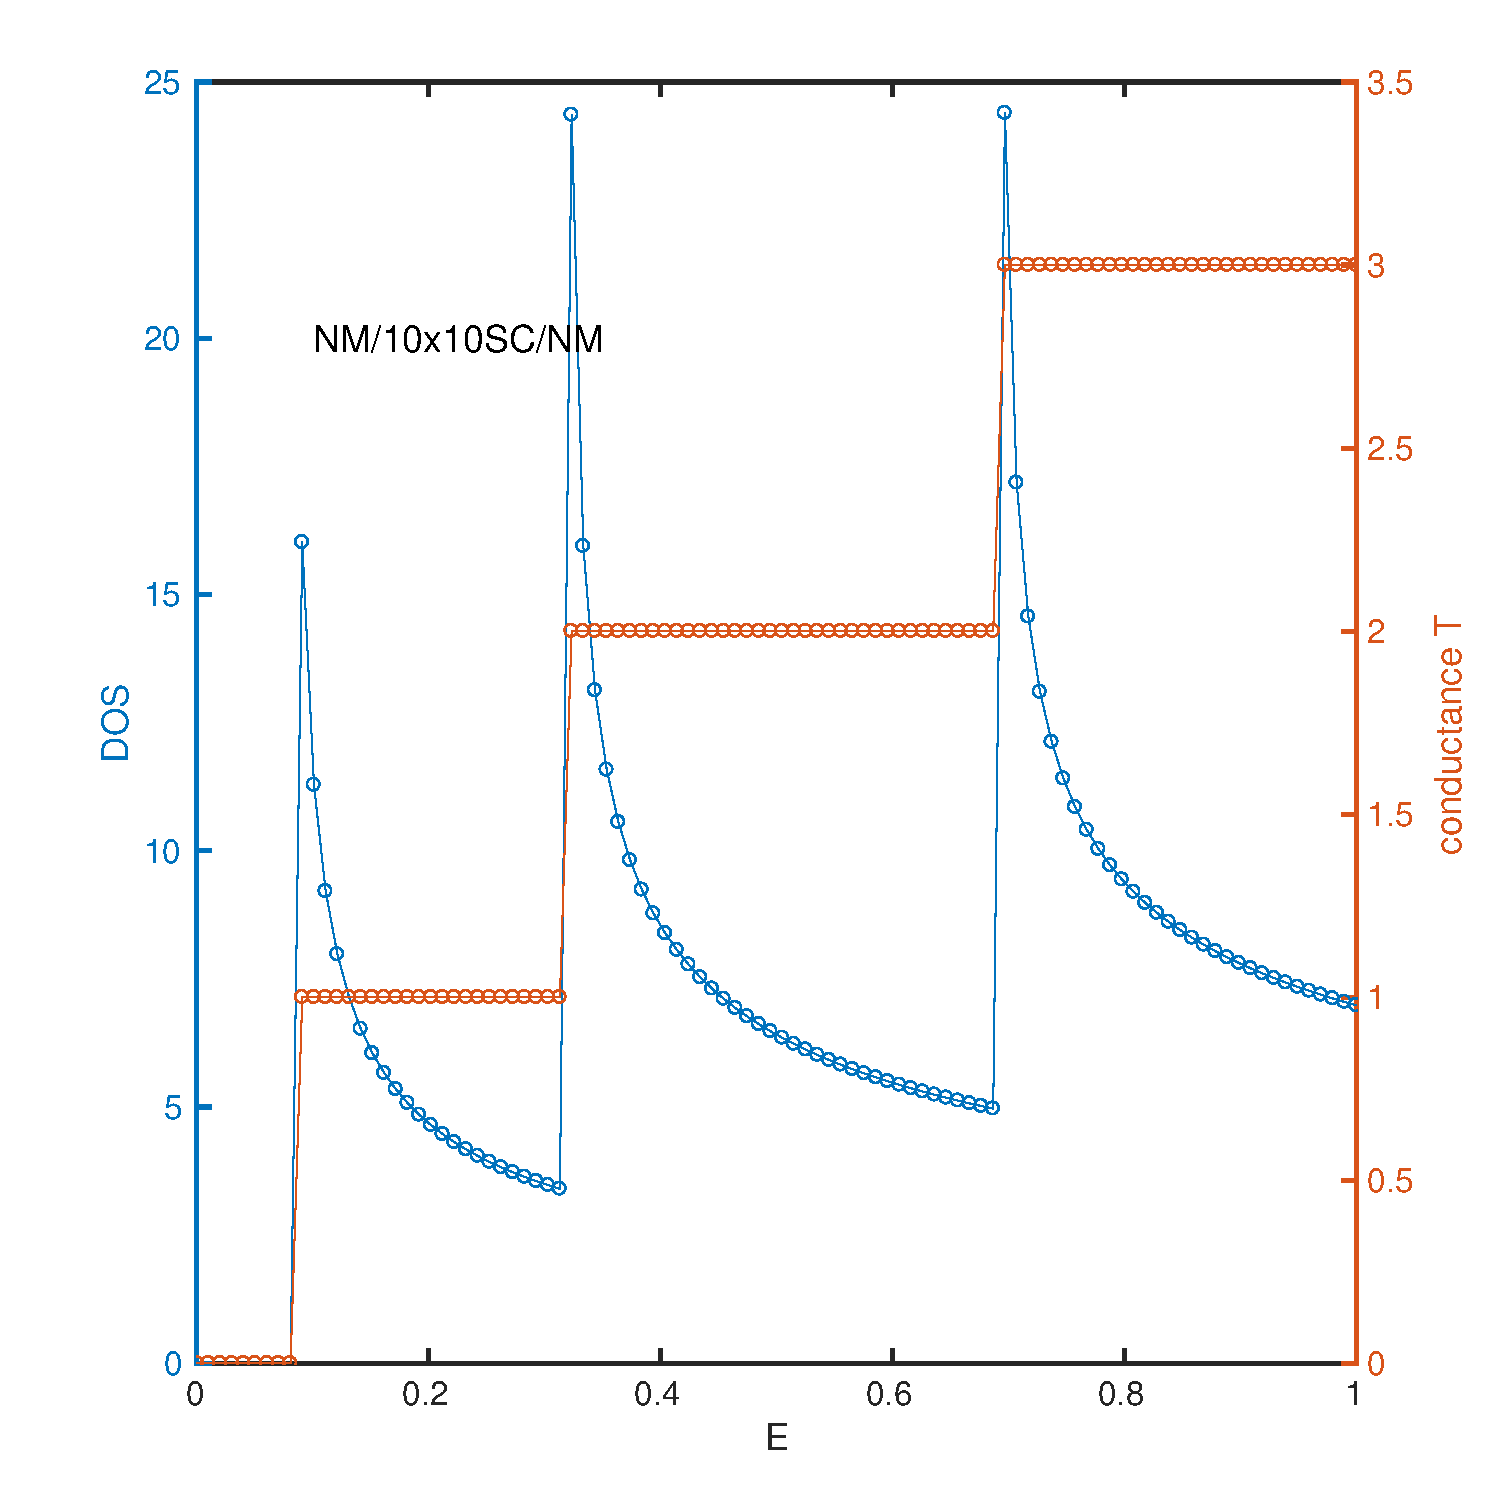
\includegraphics[width=0.5\textwidth, height=0.4\textwidth]{figures/DOST-E.pdf}
\caption{NM/10x10/NM system, 2D simple cubic lattice connected to two normal metal leads.}
\end{figure}
\subsection{NM/10x10SC/MI}
\begin{figure}[htp!]
\centering
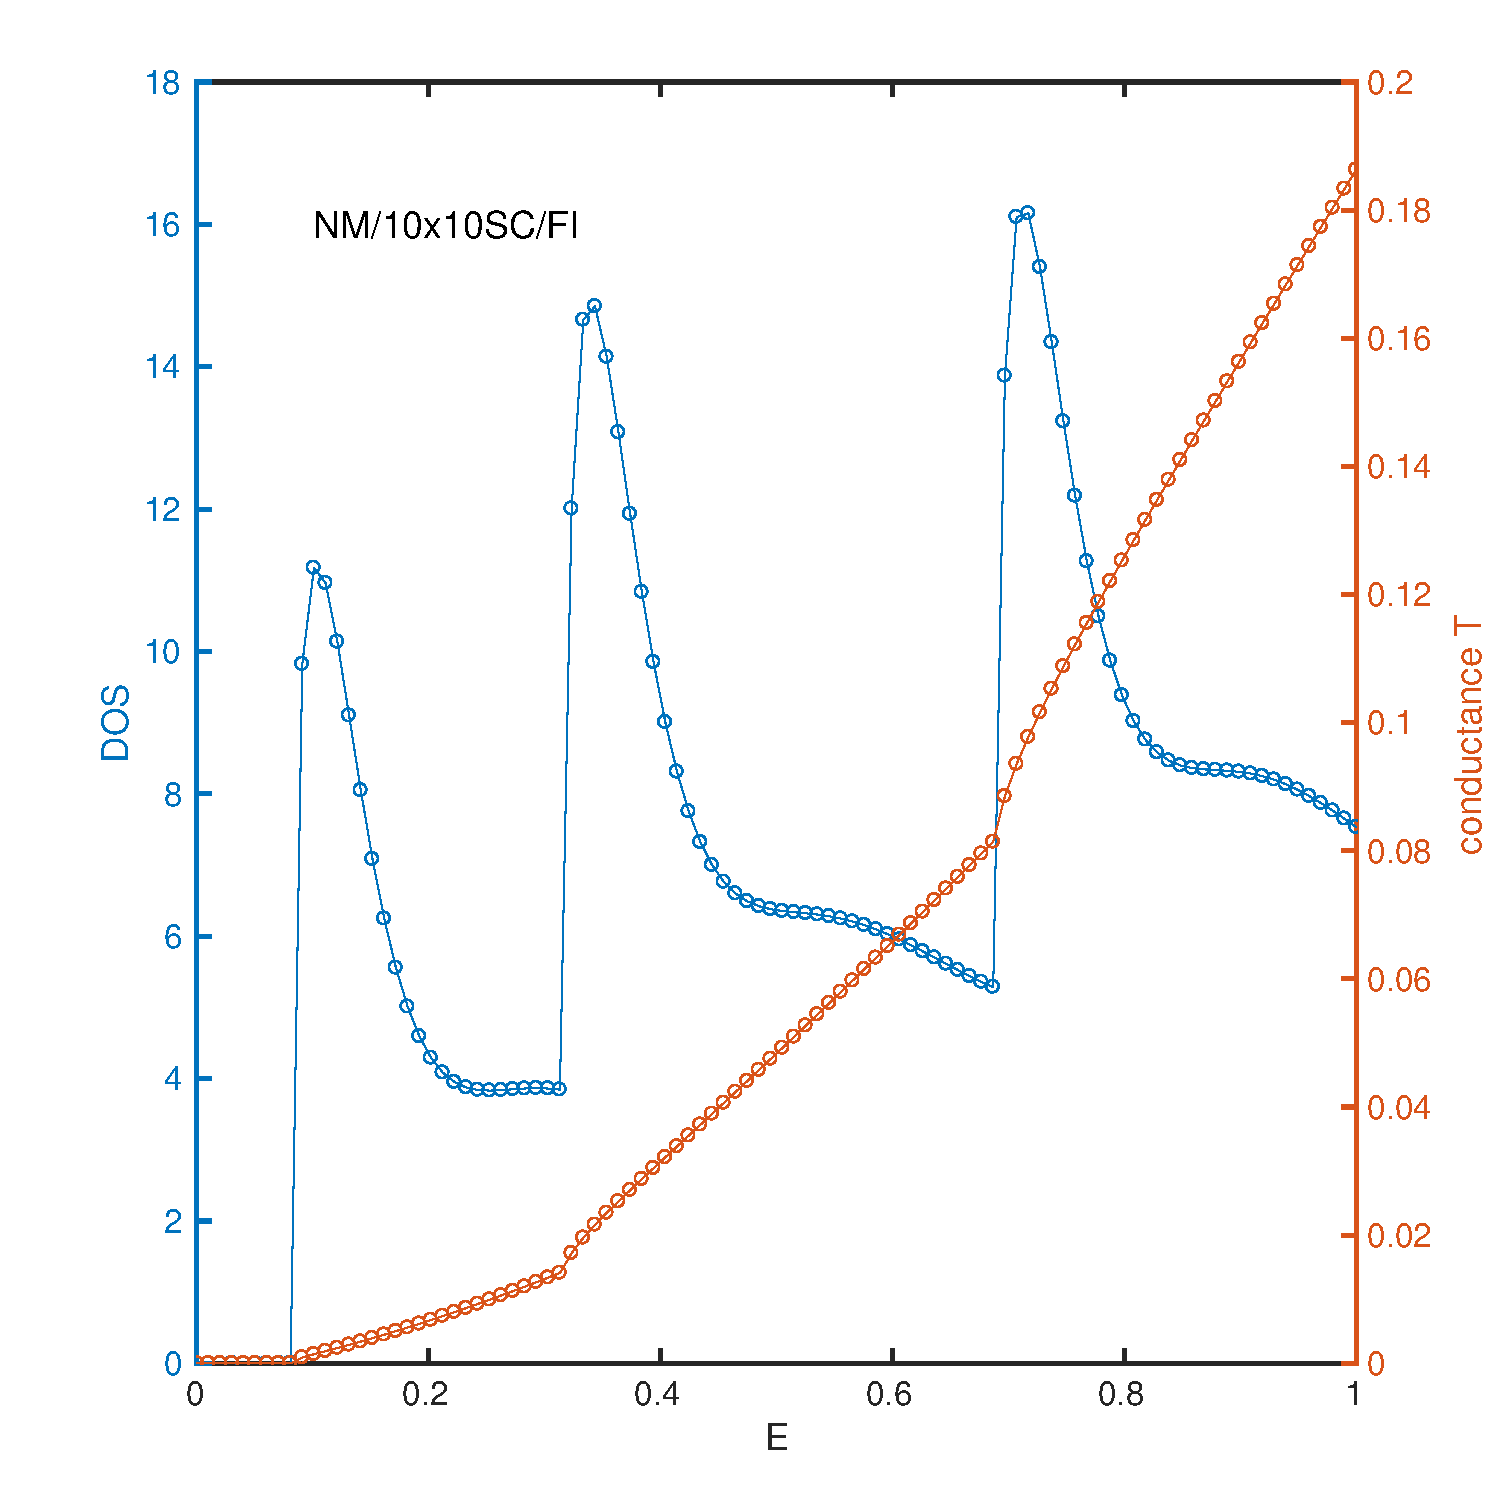
\includegraphics[width=0.5\textwidth, height=0.4\textwidth]{figures/DOST-NM-FI.pdf}
\caption{NM/10x10/MI system, 2D simple cubic lattice connected to a normal metal lead and a magnetic insulator lead with Ohmic spectra.}
\end{figure}

\subsection{Perturbation expansion of $G_{d}(\tau, \tau)$}

When neglecting left lead, the hamiltonian is
\begin{equation}
H = H_{QD} + H_{R} + H_{sd}
\end{equation}
Expand S-matrix up to the second order of J, we have
\begin{equation}
\begin{split}
&G_{d}(\tau, \tau) = -i\langle T_{C}Ss_{q}^{+}(\tau)s_{q}^{-}(\tau') \rangle \\
=& -i\sum_{k} g_{k\uparrow}(\tau', \tau) g_{k+q\downarrow}(\tau, \tau') \\
+& \int_{c}d\tau_{1}\int_{c}d\tau_{2} \sum_{kq_{1}} J_{q_{1}}^{2} g_{Rq_{1}}(\tau_{2}, \tau_{1}) g_{k\uparrow}(\tau', \tau_{2}) g_{k+q_{1}\downarrow}(\tau_{2}, \tau_{1}) g_{k\uparrow}(\tau_{1}, \tau) g_{k+q\downarrow}(\tau, \tau') \\
+& \int_{c}d\tau_{1}\int_{c}d\tau_{2} \sum_{kq_{1}} J_{q_{1}}^{2} g_{Rq_{1}}(\tau_{2}, \tau_{1}) g_{k\uparrow}(\tau', \tau) g_{k+q\downarrow}(\tau, \tau_{1}) g_{k+q-q_{1}\uparrow}(\tau_{1}, \tau_{2}) g_{k+q\downarrow}(\tau_{2}, \tau') \\
-& \int_{c}d\tau_{1}\int_{c}d\tau_{2} \sum_{kk'} J_{q}^{2} g_{Rq}(\tau_{2}, \tau_{1}) g_{k\uparrow}(\tau_{1}, \tau) g_{k+q\downarrow}(\tau, \tau_{1})  g_{k'\uparrow}(\tau', \tau_{2}) g_{k'+q\downarrow}(\tau_{2}, \tau')
\end{split}
\end{equation}

\section{Tight-binding method}
Tight-binding coupling $t$ is 
\[
t = \frac{\hbar^{2}}{2ma^{2}},
\]
in which $m$ is the effective mass of election in the lattice, assuming $m=0.08m_{e}$, which is mass of electron. $a$ is lattice distance. $\hbar = 1.0545e-34J\cdot s, m_e = 9.10938370e-31\rm{kg}$, so $t$ is in unit of $J$.

Boltzman constant $k_B = 1.3806504^{-23}J/K, e = 1.602176634^{-19}C, \hbar = 1.0545e-34J\cdot s, m_e = 9.10938370e-31\rm{kg}$
\subsection{Transportation in a electron wave guide}
An electron wave guide is a device analogous to light wave guide, in which only small number of electron wave modes can propagate. Reference to exercise 1.3 and 1.4 in S. Datta's book. For case one, in y direction, the wave guide is constrained in a hard-well potential. $U(y < -W/2) = U(y > W/2) = \infty, U(-W/2 < y < W/2) = 0$, leads to the quantization of electron states.
\begin{equation}
k_{y} = \frac{i\pi}{W}, \qquad \text{for i is integers.}
\end{equation}
$W$ is the width of wave guide and central area, $a$ is lattice constant of central lattice, $n_{\rm{wid}}$ is number of lattice points in y direction.
\begin{equation}
W = n_{\rm{wid}}\times a
\end{equation}
To get a propagate wave instead of a decaying wave, the $k_{x}$ must be a real number, or $k_{x}^{2} > 0$. The total injection energy of an election is
\begin{equation}
E = \frac{\hbar^{2} (k_{x}^{2}+k_{y}^{2})}{2m} = \frac{\hbar^{2} k_{x}^{2}}{2m} + \frac{i^{2}\hbar^{2} \pi^{2}}{2mW^{2}}.
\end{equation}
So the threshold for $i$th subband or transverse mode is
\begin{equation}
E_{i} = \frac{i^{2}\hbar^{2} \pi^{2}}{2mW^{2}},
\end{equation}
which is $0.537$ meV for first subband, effective mass $m=0.07m_{e}$, and width $W = 100nm$.




\clearpage
\section*{Appendix A: Analytic Continuation}

We list here all the analytic continuations used in this work.  For $C = AB$ (matrix multiplication), we have\cite{jauho}
\begin{gather}
C^< = A^r B^< + A^< B^a, ~~ {\rm and } ~~ C^> = A^r B^> + A^> B^a \label{conti1}
\end{gather}
and
\begin{gather}
C^r = A^r B^r , ~~ {\rm and } ~~ C^a =  A^a B^a \label{conti2}
\end{gather}
For $C(\tau,\tau') = A(\tau,\tau') B(\tau,\tau')$ or $C=A.B$ (the Hadamard matrix product), we have\cite{jauho}
\begin{gather}
C^< = A^<. B^< , ~~ {\rm and } ~~ C^> = A^> .B^> \label{conti3}
\end{gather}
and
\begin{eqnarray}
&&C^r = A^r .B^< + A^< .B^r + A^r .B^r, \nonumber \\
&& C^a = A^a .B^< + A^< .B^a + A^a. B^a \label{conti4}
\end{eqnarray}
For $C(\tau,\tau') = A(\tau,\tau') B(\tau',\tau)$ or $C = A.{\tilde B}$ where ${\tilde B}(t_1,t_2) \equiv B(t_2,t_1)$, we have\cite{jauho}
\begin{gather}
C^< = A^< .{\tilde B}^> , ~~ {\rm and } ~~ C^> = A^> .{\tilde B}^< \label{conti5}
\end{gather}
\begin{eqnarray}
&& C^r = A^< .{\tilde B}^a + A^r .{\tilde B}^< , \nonumber \\
&& C^a = A^< .{\tilde B}^r + A^a .{\tilde B}^<  \label{conti6}
\end{eqnarray}
From Eqs.~(\ref{conti5}) and (\ref{conti6}), one can easily check the relation $C^> - C^< = C^r - C^a$ which must be satisfied.


\section*{Appendix B: derivation of decoupled GF}
To show Eq.(\ref{relation1}), we follow exactly the derivation of Ref.\onlinecite{jauho} p188. We examine jth order term in the S-matrix expansion and use Wick theorem,
\begin{eqnarray}
&& \langle T_c s^+_q(\tau) a^\dagger_q(\tau') [J_q a_{q}(\tau_1) s^-_q(\tau_1) +h.c.] ...
[J_q a_{q}(\tau_j) s^-_q(\tau_j) +h.c.]\rangle \nonumber \\
&& =\langle T_c a_q(\tau_1) a^\dagger_q(\tau')\rangle J_q \langle T_c s^+_q(\tau)s^-_q(\tau_1) [J_q a_{q}(\tau_2) s^-_q(\tau_2)+h.c. ] ...
[J_q a_{q}(\tau_j) s^-_q(\tau_j) +h.c.]\rangle \nonumber \\
&&+\langle T_c a_q(\tau_2) a^\dagger_q(\tau')\rangle J_q \langle T_c s^+_q(\tau)s^-_q(\tau_2) [J_q a_{q}(\tau_1) s^-_q(\tau_1)+h.c. ] ...
[J_q a_{q}(\tau_j) s^-_q(\tau_j) +h.c.]\rangle \nonumber \\
&& + ~ {\rm remaining ~ j-2 ~ terms}
\end{eqnarray}
Note that there are j terms that are all the same. The extra factor of j combined with $(-i)^j/j!$ giving rise to $-i (-i)^{j-1}/(j-1)!$ and we can reconstruct a new S-matrix. Remember that there is a factor of $(-i)^j$ in the jth expansion of S-matrix, hence we have an extra $-i$ in S-matrix reconstruction. Notice that we did not do anything for $j=0$ term in S-matrix expansion, we then have
\begin{gather}
G_{d,R}(\tau,\tau') = g_{d,R}(\tau,\tau') + J_q \int G_d(\tau,\tau_1) g_{Rq}(\tau_1,\tau')  d\tau_1
\end{gather}
where $g_{d,R}(\tau,\tau')=-i\langle T_c s^+_q(\tau) a^\dagger_q(\tau')\rangle$ is simply zero.

\section*{Appendix C: derivation of $\Sigma_{2\sigma}^{r,<}$}
${\bar \Sigma}_{R\sigma}(\tau_1,\tau_2) =i\sum_q G_{L\bar\sigma}(\tau_1,\tau_2)\Sigma_{Rq}(\tau_2,\tau_1)$. Analytic continuation gives
\begin{gather}
{\bar \Sigma}_{R\sigma}^r(t_1,t_2) =i\sum_q G_{L\bar\sigma}^<(t_1, t_2)\Sigma_{Rq}^a(t_1, t_2) + i\sum_qG_{L\bar\sigma}^r(t_1, t_2)\Sigma_{Rq}^<(t_1, t_2),\\
\end{gather}
After a double-time Fourier transformation, we have
\begin{gather}
\int dE_1 dE_2 e^{iE_1t_1-iE_2t_2}{\bar \Sigma}_{R\sigma}^r(E_1,E_2) = i\sum_q\int dE_1 dE_2 G_{L\bar\sigma}^<(E_3, E_4)\Sigma_{Rq}^a(E_3,E_4)e^{iE_3t_1-iE_4t_2}+\cdots\\
i\sum_q G_{L\bar\sigma}^<(t_1, t_2)\Sigma_{Rq}^a(t_1, t_2) + i\sum_qG_{L\bar\sigma}^r(t_1, t_2)\Sigma_{Rq}^<(t_1, t_2),\\
\end{gather}
\begin{gather}
= i\sum_q [G_{L\bar\sigma}^r\Sigma_{L\sigma}^{<}G_{L\bar\sigma}^a](t_1, t_2)\Sigma_{Rq}^a(t_1, t_2) +i\sum_q G_{L\bar\sigma}^r(t_1, t_2)\Sigma_{Rq}^<(t_1, t_2), \\
= \sum_q [-G_{L\bar\sigma}^rf_{L\sigma}\Gamma_{L\sigma}G_{L\bar\sigma}^a\Sigma_{Rq}^a](t_1, t_2) - \sum_q G_{L\bar\sigma}^r(t_1, t_2)f_{R}\Gamma_R(t_1, t_2), \\
{\bar \Sigma}_{R\sigma}^<(t_1,t_2) =i\sum_q G_{L\bar\sigma}^<(t_1, t_2)\Sigma_{Rq}^>(t_1, t_2).
\end{gather}

\section*{Appendix C2: double-time Fourier transformation}
\begin{gather}
C(t_1, t_2) = A(t_1, t_2)B(t_1, t_2)
\end{gather}

\section*{Appendix D: continuation on Eq.~(\ref{lesser2})}
Eq.~(\ref{lesser2}) is
\begin{gather}
G_{d}(\tau,\tau') = -iG_{L\uparrow}(\tau',\tau)G_{L\downarrow}(\tau,\tau') -i G_{L\uparrow}(\tau_1,\tau)G_{L\downarrow}(\tau,\tau_1) \Sigma_{Rq}(\tau_1,\tau_2) G_{d}(\tau_2,\tau'). \label{relation5}
\end{gather}
We define
\begin{eqnarray}
% \center
A(\tau_{1}, \tau') \equiv\int d\tau_{2}\Sigma_{R }\left(\tau_{1}, \tau_{2}\right) G_{d}\left(\tau_{2}, \tau^{\prime}\right)\\
B(\tau, \tau_{1}) \equiv G_{L \uparrow}\left(\tau_{1}, \tau\right) G_{L \downarrow}\left(\tau, \tau_{1}\right)\\
C(\tau, \tau')\equiv -i G_{L \uparrow}\left(\tau_{1}, \tau\right) G_{L \downarrow}\left(\tau, \tau_{1}\right) A(\tau_{1}, \tau') \rightarrow \\
C(\tau, \tau') = -i\int d\tau_{1}B(\tau, \tau_{1})A(\tau_{1}, \tau')\\
D(\tau, \tau') \equiv -i G_{L \uparrow}\left(\tau^{\prime}, \tau\right) G_{L \downarrow}\left(\tau, \tau^{\prime}\right)
\end{eqnarray}
So, we have
\begin{equation}
G_{d}(\tau, \tau') = D + C
\end{equation}
Using the analytic continuation theorem, we have
\begin{equation}
D^{<} = -i G_{L \uparrow}^{>} G_{L \downarrow}^{<}
\end{equation}
\begin{equation}
C^{<}=-i(B^{r} A^{<}+B^{<} A^{a})
\end{equation}
where
\begin{equation}
B^{r} = G_{L \uparrow}^{a} G_{L \downarrow}^{<}+G_{L \uparrow}^{>} G_{L \downarrow}^{r}+G_{L \uparrow}^{a} G_{L \downarrow}^{r}
\end{equation}
\begin{equation}
A^{<}=\Sigma_{R}^{r} G_{d}^{<}+\Sigma_{R}^{<} G_{d}^{a}
\end{equation}
\begin{equation}
B^{<}=G_{L\uparrow}^{>} G_{L\downarrow}^{<}
\end{equation}
\begin{equation}
A^{a}=\Sigma_{R}^{a} G_{d}^{a}
\end{equation}
Then, the analytic continuation theorem on Eq.(\ref{lesser1}) yields
\begin{equation}
G_{d}^{<}=-i G_{L \uparrow}^{>} G_{L \downarrow}^{<} -i\left[(G_{L \uparrow}^{a} G_{L \downarrow}^{<}+G_{L \uparrow}^{>} G_{L \downarrow}^{r}+G_{L \uparrow}^{a} G_{L \downarrow}^{r})(\Sigma_{R}^{r} G_{d}^{<}+\Sigma_{R}^{<} G_{d}^{a}) + (G_{L\uparrow}^{>} G_{L\downarrow}^{<})(\Sigma_{R}^{a} G_{d}^{a})\right]
\label{eq:Gd<}
\end{equation}
Similarly, 
\begin{equation}
\begin{split}
C^{r}&=-iB^{r} A^{r} \\
&=-i(G_{L \uparrow}^{a} G_{L \downarrow}^{<}+G_{L \uparrow}^{>} G_{L \downarrow}^{r}+G_{L \uparrow}^{a} G_{L \downarrow}^{r})(\Sigma_{R}^{r} G_{d}^{r})
\end{split}
\end{equation}
\begin{equation}
D^{r}=-i(G_{L \uparrow}^{a} G_{L \downarrow}^{<}+G_{L \uparrow}^{>} G_{L \downarrow}^{r}+G_{L \uparrow}^{a} G_{L \downarrow}^{r}),
\end{equation}
we have
\begin{equation}
\begin{split}
G_{d}^{r} &=  -i(G_{L \uparrow}^{a} G_{L \downarrow}^{<}+G_{L \uparrow}^{>} G_{L \downarrow}^{r}+G_{L \uparrow}^{a} G_{L \downarrow}^{r})-i(G_{L \uparrow}^{a} G_{L \downarrow}^{<}+G_{L \uparrow}^{>} G_{L \downarrow}^{r}+G_{L \uparrow}^{a} G_{L \downarrow}^{r})(\Sigma_{R}^{r} G_{d}^{r}) \\
&=\frac{-i\left(G_{L \uparrow} G_{L \downarrow}\right)^{r}}{ 1+i\left(G_{L \uparrow} G_{L \downarrow}\right)^{r} \Sigma_{R}^{r}}
\end{split}
\end{equation}
\begin{equation}
(G_{L \uparrow} G_{L \downarrow})^{r} \equiv G_{L \uparrow}^{a} G_{L \downarrow}^{<}+G_{L \uparrow}^{>} G_{L \downarrow}^{r}+G_{L \uparrow}^{a} G_{L \downarrow}^{r}
\end{equation}
Now we calculate $G_{d}^{a}$.
\begin{equation}
C^{a}=-iB^{a} A^{a}
\end{equation}
\begin{equation}
B^{a}=G_{L \uparrow}^{r} G_{L \downarrow}^{<}+G_{L \uparrow}^{>} G_{L \downarrow}^{a}+G_{L \uparrow}^{r} G_{L \downarrow}^{a}
\end{equation}
\begin{equation}
D^{a}=-i(G_{L \uparrow}^{r} G_{L \downarrow}^{<}+G_{L \uparrow}^{>} G_{L \downarrow}^{a}+G_{L \uparrow}^{r} G_{L \downarrow}^{a})
\end{equation}
So we have
\begin{equation}
G_{d}^{a} = -i(G_{L \uparrow}^{r} G_{L \downarrow}^{<}+G_{L \uparrow}^{>} G_{L \downarrow}^{a}+G_{L \uparrow}^{r} G_{L \downarrow}
^{a})-i(G_{L \uparrow}^{r} G_{L \downarrow}^{<}+G_{L \uparrow}^{>} G_{L \downarrow}^{a}+G_{L \uparrow}^{r} G_{L \downarrow}^{a})(\Sigma_{R}^{a} G_{d}^{a})
\end{equation}
From Eq.(\ref{eq:Gd<}) we have
\begin{equation}
\begin{split}
G_{d}^{<}&=-i G_{L \uparrow}^{>} G_{L \downarrow}^{<}\left(1+\Sigma_{R}^{a} G_{d}^{a}\right)-i\left(G_{L \uparrow} G_{L \downarrow}\right)^{r}\left(\Sigma_{q}^{<} G_{d}^{a}+\Sigma_{R}^{r} G_{d}^{<}\right)\\
&=\frac{-i G_{L \uparrow}^{>} G_{L \downarrow}^{<}\left(1+\Sigma_{R}^{a} G_{d}^{a}\right) - i\left(G_{L \uparrow} G_{L \downarrow}\right)^{r}\Sigma_{R}^{<} G_{d}^{a}}{1+i\left(G_{L \uparrow} G_{L \downarrow}\right)^{r}\Sigma_{R}^{r}} \\
&=\frac{-i G_{L \uparrow}^{>} G_{L \downarrow}^{<}\left(1+\Sigma_{R}^{a} G_{d}^{a}\right)}{1+i\left(G_{L \uparrow} G_{L \downarrow}\right)^{r}\Sigma_{R}^{r}} + G_{d}^{r}\Sigma_{R}^{<} G_{d}^{a}\\
&=-i(G_{d}^{r}\Sigma_{R}^{r}+1) G_{L \uparrow}^{>} G_{L \downarrow}^{<}\left(1+\Sigma_{R}^{a} G_{d}^{a}\right) + G_{d}^{r}\Sigma_{R}^{<} G_{d}^{a}
\end{split}
\end{equation}
Similarly,
\begin{equation}
G_{d}^{>}=-i\left(G_{d}^{r} \Sigma_{R}^{r}+1\right) G_{L \uparrow}^{<} G_{L \downarrow}^{>}\left(1+\Sigma_{R}^{a} G_{d}^{a}\right)+G_{d}^{r} \Sigma_{R}^{>} G_{d}^{a}
\end{equation}

\section*{Appendix E: derivation on Eq.~(\ref{Gd-dn})}
\begin{eqnarray}
G_{d\downarrow}(\tau,\tau') =G_{L\downarrow}(\tau,\tau') + i\sum_q G_{L\downarrow}(\tau,\tau_1)  G_{L\uparrow}(\tau_1,\tau_2)\Sigma_{Rq}(\tau_2,\tau_1) G_{L\downarrow}(\tau_2,\tau'),\\
G_{r\downarrow}^r(t,t') =G_{L\downarrow}^r(t,t') + ???
\end{eqnarray}








\begin{thebibliography}{10}
\bibitem{ref1}
Y, K, Kato. Observation of the Spin Hall Effect in Semiconductors[J]. Science, 2004.
\bibitem{Jauho}
Antti-Pekka Jauho, Quantum Kinetics in Transport and Optics of Semiconductors, P188.
\bibitem{Wu} L. Gu, H. H. Fu, and R. Q. Wu, Phys. Rev. B 94, 115433 (2016).
\bibitem{Ren} J. Ren, Phys. Rev. B 88, 220406 (2013).
\end{thebibliography}


% \end{CJK}
\end{document}


